%%
%% Copyright 2007, 2008, 2009 Elsevier Ltd
%%
%% This file is part of the 'Elsarticle Bundle'.
%% ---------------------------------------------
%%
%% It may be distributed under the conditions of the LaTeX Project Public
%% License, either version 1.2 of this license or (at your option) any
%% later version.  The latest version of this license is in
%%    http://www.latex-project.org/lppl.txt
%% and version 1.2 or later is part of all distributions of LaTeX
%% version 1999/12/01 or later c.
%%
%% The list of all files belonging to the 'Elsarticle Bundle' is
%% given in the file `manifest.txt'.
%%

%% Template article for Elsevier's document class `elsarticle'
%% with harvard style bibliographic references
%% SP 2008/03/01
%%
%%
%%
%% $Id: elsarticle-template-harv.tex 4 2009-10-24 08:22:58Z rishi $
%%
%%
\documentclass[preprint,authoryear,12pt]{elsarticle}

%% Use the option review to obtain double line spacing
%% \documentclass[authoryear,preprint,review,12pt]{elsarticle}

%% Use the options 1p,twocolumn; 3p; 3p,twocolumn; 5p; or 5p,twocolumn
%% for a journal layout:
%% \documentclass[final,authoryear,1p,times]{elsarticle}
%% \documentclass[final,authoryear,1p,times,twocolumn]{elsarticle}
%% \documentclass[final,authoryear,3p,times]{elsarticle}
%% \documentclass[final,authoryear,3p,times,twocolumn]{elsarticle}
%% \documentclass[final,authoryear,5p,times]{elsarticle}
%% \documentclass[final,authoryear,5p,times,twocolumn]{elsarticle}

%% if you use PostScript figures in your article
%% use the graphics package for simple commands
%% \usepackage{graphics}
%\usepackage{cases}
%% or use the graphicx package for more complicated commands
\usepackage{graphicx}
%% or use the epsfig package if you prefer to use the old commands
\usepackage{epsfig}

\usepackage{comment}

\usepackage{epstopdf}

\usepackage{bm}
\usepackage{hyperref,url}
\hypersetup{colorlinks=true, urlcolor=blue, linkcolor=blue, citecolor=red}

%\usepackage[obeyFinal]{todonotes}
\usepackage{todonotes}
\newcommand{\jrp}[1]{\todo[color=blue!30, size=\small]{JRP: #1}}
\newcommand{\JGnote}[1]{\fbox{\parbox{\textwidth}{ \color{blue} JG: #1}}}

%% The amssymb package provides various useful mathematical symbols
\usepackage{amssymb,amsmath,array}
%% The amsthm package provides extended theorem environments
%% \usepackage{amsthm}

%% The lineno packages adds line numbers. Start line numbering with
%% \begin{linenumbers}, end it with \end{linenumbers}. Or switch it on
%% for the whole article with \linenumbers after \end{frontmatter}.
%% \usepackage{lineno}

%% natbib.sty is loaded by default. However, natbib options can be
%% provided with \biboptions{...} command. Following options are
%% valid:

%%   round  -  round parentheses are used (default)
%%   square -  square brackets are used   [option]
%%   curly  -  curly braces are used      {option}
%%   angle  -  angle brackets are used    <option>
%%   semicolon  -  multiple citations separated by semi-colon (default)
%%   colon  - same as semicolon, an earlier confusion
%%   comma  -  separated by comma
%%   authoryear - selects author-year citations (default)
%%   numbers-  selects numerical citations
%%   super  -  numerical citations as superscripts
%%   sort   -  sorts multiple citations according to order in ref. list
%%   sort&compress   -  like sort, but also compresses numerical citations
%%   compress - compresses without sorting
%%   longnamesfirst  -  makes first citation full author list
%%
%% \biboptions{longnamesfirst,comma}

% \biboptions{}

%\journal{Computer Methods in Applied Mechanics and Engineering}
\journal{Comput Meth Appl Mech Eng}
\newcommand{\frc}{\displaystyle\frac}
\newcommand{\PN}[2][error]{P$_{#1}$DG-P$_{#2}$}

\begin{document}



\begin{frontmatter}

%% Title, authors and addresses

%% use the tnoteref command within \title for footnotes;
%% use the tnotetext command for the associated footnote;
%% use the fnref command within \author or \address for footnotes;
%% use the fntext command for the associated footnote;
%% use the corref command within \author for corresponding author footnotes;
%% use the cortext command for the associated footnote;
%% use the ead command for the email address,
%% and the form \ead[url] for the home page:
%%
%% \title{Title\tnoteref{label1}}
%% \tnotetext[label1]{}
%% \author{Name\corref{cor1}\fnref{label2}}
%% \ead{email address}
%% \ead[url]{home page}
%% \fntext[label2]{}
%% \cortext[cor1]{}
%% \address{Address\fnref{label3}}
%% \fntext[label3]{}

\title{The Overlapping Control Volume Finite Element Method for Multiphase Porous Media Flow Modelling \\
Part I: Numerical Formulation}

%% use optional labels to link authors explicitly to addresses:
\author[UoA]{J.L.M.A. Gomes}\corref{cor1}\ead{jefferson.gomes@abdn.ac.uk} \author[IC]{D. Pavlidis} 
\author[IC]{J.R. Percival} \author[NSW]{P. Mostaghimi} \author[IC,NORMS]{P. Salinas} \author[IC]{Z. Xie} 
\author[IC]{C.C. Pain} \author[NORMS]{M.D. Jackson}
%\author[IC]{M. Blunt}

\cortext[cor1]{Corresponding author.}
\address[UoA]{Environmental and Industrial Fluid Mechanics Group, School of Engineering, University of Aberdeen, UK}
\address[IC]{Applied Modelling and Computation Group, Department of Earth Science and Engineering, Imperial College London, UK}
\address[NSW]{School of Petroleum Engineering, University of New South Wales, Australia}
\address[NORMS]{Novel Reservoir Modelling and Simulation Group, Department of Earth Science and Engineering, Imperial College London, UK}

\begin{abstract} 
This is the first of two papers devoted to a novel finite element method formulation to solve subsurface multi-fluid flows. The overlapping control volume finite element method (OCVFEM) has two major strengths, firstly it uses a dual consistent pressure-velocity representation in control volume and finite element spaces which ensures local mass conservation. Secondly, it uses a family of finite element types that ensures multiphase Darcy equations can be exactly enforced. The underlying mass conservation equations are solved in control volume space and finite elements are used to obtain high-order fluxes on control volume boundaries. The novelty of the method lies in (a) permitting both continuous and discontinuous description of pressures and saturations between elements; (b) the use of arbitarily high-order polynomial representation for pressure and velocity within the mixed formulation; (c) the use of high-order flux-limited methods to avoid introducing non-physical oscillations as well as achieving high-order time accuracy where and when possible. In this paper, the new model is described and test cases are introduced to show the numerical accuracy in one- and two-dimensional simulations. More extensive applications are introduced in the second part of this two part paper. 
\end{abstract}

\begin{keyword} %% keywords here, in the form: keyword \sep keyword
Multi-fluid flows \sep Darcy equations \sep Porous media \sep Finite element methods \sep Mixing formulation \sep Discontinuous Galerkin.


\end{keyword}

\end{frontmatter}

%\tableofcontents
%\linenumbers

\clearpage
%%%         %%%
%%% SECTION %%%
%%%         %%%
\section{Introduction}
Numerical modelling of multiphase flow in porous media has applications in a wide range of disciplines from hydrocarbon and groundwater exploration and safety assessment of deep geological disposal of radioactive waste to CO$_{\text{2}}$ migration and trapping mechanisms in carbon capture and storage (CCS) operations~\citep{chen_2006, aiea_1999, pruess_1990c, jiang_2011}. Complex geometries with irregular (and often internal) boundaries and heterogeneous geological formations are some of the main challenges to accurately simulate such flows.

Finite difference methods (FDM) have been extensively used in modelling and simulation of fluid flows in porous media~\citep{aziz_1986, chen_1997, chen_2005} however, they are strongly dependent on mesh quality and orientation and cannot easily represent complex geometries. In addition, FDM produce excessive numerical dispersion in heterogeneous porous matrix \citep{chavent_1986}. The geometrical flexibility of finite element methods (FEM) has proven to overcome these deficiencies. Among FEM-based formulations for porous media, the control volume finite element method (CVFEM) has become increasingly popular as it can guarantee local mass conservation and high-order numerical accuracy as well as being able to use tetrahedral geometry-conforming elements~\citep{forsyth_1990, cordazzo_2004, geiger_2004, hurtado_2007}.  \citet{huber_2000} demonstrated that the vertex-centred finite volume - finite element method (or Box scheme) can achieve similar goals~\citep[see also][]{helmig_1997}.

%For porous media flows, CVFEM discretisations with Galerkin-FEM formulation for the pressure equation has been used to solve Darcy and Richard equations as described by \citet{fung_1992} and \citet{cumming_2011}. 
\citet{durlofsky_1993,durlofsky_1994} compared the performance of a mixed FEM formulation (i.e., piecewise constant in pressure and piecewise linear in velocity) and the classical CVFEM for single phase Darcy flows. He concluded that the latter is more computationally efficient and numerically accurate than the former for problems involving a (relatively) small number of degrees of freedom. For complex discontinuous and heterogeneous problems, mixed FEM formulations often lead to physically realistic solutions.

\medskip

CVFEM often requires high resolution meshes in regions where material properties vary abruptly, such as permeability contrasts at fracture-matrix interfaces. Since the structural geometries are captured by finite elements (FE), constructed control volumes (CV) typically extend over the interfaces which may present different properties. Therefore, some average value of the permeability (defined in the FE space but projected into the CV space) is applied across the CV's at these interface. This often leads to excessive numerical dispersion, especially in highly heterogeneous media. In order to overcome this deficiency, \citet{nick_2011b, nick_2011a} developed a new discretisation scheme -- discontinuous hybrid finite element finite volume method (DFEFVM), where CV's split along the interfaces of different material properties. This scheme was designed to simulate single and multiphase flows through discrete fractured rocks. 

\citet{cumming_2011} demonstrated that CVFEM-based discretisation could be used to solve Richards' equations (coupled mass conservation and Darcy equations) in heterogeneous porous media with relatively small computational overhead, compared with traditional coupled velocity-pressure based formulations. Fluxes over CV's were calculated based upon material properties, whereas saturation fields were volume-averaged at the interface of the materials, enforcing mass balance as described by \citet{kirkland_1992}~\citep[see also][]{forsyth_1990,cumming_phd2012}.

\medskip

Discontinuity-capturing schemes~\citep[e.g., shock waves, contact surface or material discontinuity -- see][]{brooks_1982,tezduyar_1986} were originally developed to resolve sharp changing of field variables. Related discontinuity-capturing schemes include the discontinuous-Galerkin FEM (DGFEM) scheme in which continuity of the solution is not explicitly enforced, allowing sharp gradients in the solution fluxes to be captured. The DG formulation is a stabilised finite element method that is (a) locally conservative, (b) designed to achieve high-order accuracy, and (c) used in a wide range of Reynolds numbers applications. DGFEM solution fields are allowed to be discontinuous at the element faces, thus the flow solution is able to naturally handle discontinuities at material interfaces. In addition, DGFEM is well-suited to deal with interface problems by incorporating specially-designed interface fluxes. These properties have attracted the attention of subsurface flow research communities in the past 15 years \citep[see][]{riviere_2000,riviere_2002,bastian_2002}.

\medskip 

In this paper, we describe a novel overlapping CVFEM (or OCVFEM) discretisation which is conservative and consistent \citep{jackson_2013}. The continuity equations are embedded into the pressure equation to enforce mass conservation and exact force balance. This is possible by using dual CV and FEM discretisations for the pressure equation, while saturation is discretised in CV space. The overall formulation employs an implicit algorithm with respect to time that is unconditionally stable for pure advection and with no restriction on the time-step size.

The formulation has two key developments. Firstly, it uses a dual consistent pressure-velocity representation in CV and FEM spaces embedded in a  family of triangular and tetrahedral finite element-pairs, P$_{n}$DG-P$_{m}$[DG] \citep[see][]{cotter_2009b}. In this element type, the dual velocity and pressure fields are represented by $n^{\rm th}$ order (discontinuous) and $m^{\rm th}$ order (continuous/discontinuous) polynomials, respectively. This allows the velocity to exactly represent pressure gradients in the flow solution for homogeneous material properties. 
The P$_{n+1}$DG-P$_{n}$DG element-pair, which has similar properties to the P$_n$DG-P$_{n+1}$ element-pair, allows a representation in which pressure, %\jrp{Saturation is on the control volume space and thus always discontinuous} 
saturation and other solution variables are all fully discontinuous across finite element boundaries. The second key development is that this formulation uses an overlapping finite element representation of velocity within each element. This approach can achieve an exact representation of the Darcy force balance equations. 

\medskip
This is the first of two papers on the proposed methodology. Here we focus on model description and initial validation, whereas in the second part~\citep{pavlidis_2013} we employ the numerical formulation for a number of multiphase porous media flow simulations to demonstrate numerical accuracy and convergence rates. The remainder of this paper is organised as follows. New element types and the overlapping formulation are introduced in Sections~\ref{element_types_section} and~\ref{overlapping_method_section}.  A detailed description of the new porous media methods is given in Section~\ref{transport_methods_section}. Scalar field equations, upwinding schemes and solution methods are introduced in Sections~\ref{Section:Saturation_Global}-\ref{Section:SolvingLinearEqns}. Initial model validation is presented in Section~\ref{Section:Results} and final remarks are drawn in Section~\ref{conc}.


%%%         %%%
%%% SECTION %%%
%%%         %%%
\section{Continuous and Discontinuous Finite Element Types and Control Volumes} \label{element_types_section}
The family of P$_{n}$DG-P$_{n+1}$ element-pairs was originally introduced by \citet{cotter_2009a} for geophysical fluid dynamics applications \citep[see also][]{cotter_2012}. In particular, the P$_{1}$DG-P$_{2}$ element-pair was originally developed to represent the balance of geostrophic pressure and velocity without introducing spurious pressure modes. This element-pair uses element-wise linear polynomial FE basis functions, discontinuous across element interfaces for velocity $\left(\text{P}_{1}\text{DG}\right)$, and quadratic polynomial finite element basis functions for pressure which maintain $C_{\text{0}}$ continuity across element boundaries $\left(\text{P}_{2}\right)$. %This is analogous to the exact balance also achieved with this element between the frictional and pressure gradient terms in Darcy's equations.

Figure~\ref{fem_cv_represent_a} displays three element types of the P$_{n}$DG-P$_{n+1}$ family that are used in this set of papers. P$_{\text{0}}$DGP$_{\text{1}}$ and P$_{1}$DG-P$_{2}$ are shown in Fig.~\ref{fem_cv_represent_a}(a) and (b), respectively, where pressure nodes are stored in the vertices and edges (in P$_{\text{2}}$ elements) of triangular/tetrahedral elements and control volumes are constructed around them based on a Voronoi decomposition.  One can realise that due to the continuous finite element node structure, control volumes span more than one element. Having CV's spanning to multiple elements may create artificial diffusion in cases where there are large variations in physical properties across elements, such as at the boundary between materials with different absolute permeabilities. As an alternative, two families of fully discontinuous element-pairs are also considered: P$_{n}$DG-P$_{n}$DG and P$_{n+1}$DG-P$_{n}$DG~\citep[Fig.~\ref{fem_cv_represent_a}(c), applications using these element-pairs are exploited in][]{pavlidis_2015} along with control volumes from their dual Voronoi decompositions. These families of element-pairs are LBB stable and free from chequerboard pressure modes, as previously demonstrated by~\citet{cotter_2009b}~\citep[see also][]{cotter_2011}.

%\begin{center}
%\JGnote{Most of the simulations in this paper (and the next) were performed using P$_{1}$DGP$_{2}$ elements. However it seems that the sketch of this element-pair was deleted/replaced by P$_{0}$DGP$_{1}$ and by the double-discontinuous element (fig.1 left/right) -- was this replacement on purpose or was it a mistake?} 
%\end{center}

%%%         %%%
%%% SECTION %%%
%%%         %%%
\section{Overlapping-CVFEM Formulation -- An Accurate Representation of Multiphase Darcy Flows}
\label{overlapping_method_section}
Darcy's law for immiscible multiphase flow may be written \citep{chen_2006} in the form:%,bear_1972}:
\begin{equation}\label{e:darcy_eqn}
  \mathbf{q}_{\alpha} = -\frac{\mathcal{K}_{{r}_\alpha}\mathbf{K}}{\mu_{\alpha}}\left( \nabla p_{\alpha} - {\mathbf{s}_{u}}_{\alpha} \right),
\end{equation}
where $\mathbf{q}_{\alpha}=\left(q_\alpha^{(1)},q_\alpha^{(2)},q_\alpha^{(3)}\right)^{\text{T}}$ is the $\alpha$-th phase Darcy flow rate for 3D flows, $\mathbf{K}$ is the absolute permeability tensor of the porous matrix, $\mathcal{K}_{{r}_\alpha}\left(S_{\alpha}\right)$ is the phase relative permeability, which is a function of the phase saturation $S_{\alpha}\left(\mathbf{r},t\right)$. $\mu_{\alpha}$, $p_{\alpha}$ and $\mathbf{s}_{{u}_\alpha}$ are the phase dynamic viscosity, pressure and a source term, respectively.

If we define the interstitial or advective phase velocity, averaged over the entire medium, as $\mathbf{u}_\alpha= \mathbf{q}_\alpha/S_\alpha$, then we may rewrite Eqn.~\ref{e:darcy_eqn} as:
\begin{equation}
  \bm{v}_\alpha:= {\underline {\underline \sigma}}_{\alpha} \mathbf{u}_{\alpha} = - \nabla p + {\mathbf{s}_{u}}_{\alpha},
  \label{force-bal}
\end{equation}
where ${\underline {\underline \sigma}}_{\alpha}=\mu_\alpha S_\alpha \left(\mathcal{K}_{{r}_\alpha}\mathbf{K}\right)^{-1}$ represents the implicit linearisation of the viscous frictional forces and $\bm{v}_\alpha$ is a saturation averaged vector of the force density of the phase, related to the advective velocity through $\bm{u}_\alpha={\underline {\underline \sigma}}_{\alpha}^{-1}\bm{v}_\alpha$.% arising in the derivation of extended Darcy's law.

In order to discretise Eqn.~\ref{force-bal}, we assume a finite element representation for the force and pressure fields and a control volume representation for phase saturation fields. The representations for force density and pressure in terms of their FE basis functions $Q_{j}$ and $P_{j}$  may be expressed, respectively, as:
\begin{displaymath}
  \bm{v}_\alpha(\bm{r},t) = \sum\limits_{j=1}^{\mathcal{N}_u} Q_{j}(\bm{r})\bm{v}_{\alpha,j}(t) \;\;\;\;\text{ and } \;\;\;\; p(\bm{r},t)  = \sum\limits_{j=1}^{\mathcal{N}_p} P_{j}(\bm{r})p_{j}(t).
\end{displaymath} 
Here $\mathcal{N}_{u}$ and $\mathcal{N}_{p}$ are the total number of degrees of freedom for the FE force and pressure representations. Each component of the weak form of the force balance (Eqn.~\ref{force-bal}) is tested with the force density basis function space to obtain:
\begin{eqnarray}
  \sum\limits_{E} \left. \int\limits_{\Omega_E} { {Q}}_i
   \left ( {\mathbf v}_\alpha + \nabla p
  -{\mathbf s}_{u_\alpha} \right) dV \right. + \displaystyle
  \oint_{\Gamma_{E}} {Q}_i {\mathbf n} \left(p - \tilde{p}\right) d\Gamma
  + \nonumber \\ 
  \oint_{\Gamma_{\Omega}} { Q}_i {\mathbf n} \left(p -
  p_{bc}\right) d\Gamma = \bm{0},
  \label{force-semi-disc} 
\end{eqnarray} 
where $\Omega_E$ and $\Gamma_{E}$ are the volume and boundary of element $E$, respectively, and $\Gamma_{\Omega}$ is the boundary of the computational domain. The numerical pressure appearing in the jump condition, $\tilde{p}$, is an average of the potentially discontinuous pressure across the element $E$,
\[\tilde{p}=\lim_{a\rightarrow 0} 
   \frac{1}{2}\left[p(\bm{r}+a\bm{n})+p(\bm{r}-a\bm{n})\right].\] This term therefore vanishes when pressure is continuous. Equation ~\ref{force-semi-disc} can be represented, in matrix form, as:
\begin{equation}
  {\mathbf M} \underline {\mathbf v} = -{\mathbf C} \underline {\mathbf p} + \underline {\mathbf s}_{u}, \label{force-balance-matrix-form}
\end{equation}
where the velocity $\left(\underline{\bf v}\right)$ and pressure $\left(\underline{\bf p}\right)$ solution-vectors are defined as,
\begin{eqnarray}
  &&\underline{{\bf v}} = \left({v_x}_{1,1},\ldots,{v_x}_{\mathcal{N}_\alpha,
    \mathcal{N}_u}, {v_y}_{1,1},\ldots,{v_y}_{\mathcal{N}_\alpha,
    \mathcal{N}_u},{v_z}_{1,1},\ldots,{v_z}_{\mathcal{N}_\alpha,
    \mathcal{N}_u}\right)^{T} \;\;\;\;\text{and} \nonumber \\ &&
  \underline{{\bf p}} = \left(p_1, p_2, p_3, ...,
  p_{\mathcal{N}_p}\right)^T. \nonumber \nonumber
\end{eqnarray}
$\mathcal{N}_{\alpha}$ is the number of phases and $v_x$, $v_y$, $v_z$ are the the velocity components associated with the $x-$ and $y-$ and $z-$ coordinates, respectively. 

Finally, the mass matrix ${\mathbf M}$, gradient matrix
${\mathbf C}$ and discretised source term ${\mathbf s}_{u}$ are:
\[\mathbf{M}=\left(
\begin{array}{ccc}
  \bm{M}^{(1,1)} &\bm{0} &\bm{0} \\
  \bm{0}   &\bm{M}^{(2,2)} &\bm{0} \\
  \bm{0} &\bm{0}  &\bm{M}^{(3,3)}   
\end{array}\right),\]
\[
\bm{C}=\left(
\begin{array}{ccc}
  \bm{C}^{(1,1)}&\bm{0}&\bm{0}\\
  \bm{0}&\bm{C}^{(2,2)}&\bm{0}\\
  \bm{0}&\bm{0}&\bm{C}^{(3,3)}\\
\end{array}\right)\quad \text{ and } \;\;
\bm{s}_u=\left(
\begin{array}{ccc}
  \bm{s}^{(1,1)}&\bm{0}&\bm{0}\\
  \bm{0}&\bm{s}^{(2,2)}&\bm{0}\\
  \bm{0}&\bm{0}&\bm{s}^{(3,3)}\\
\end{array}\right),\quad
\]
with blocks defined by:
\begin{eqnarray}
  && \left[{\mathbf M}^{(i,j)}\right]_{p,q} = \int_{\Omega}  Q_{p} \delta_{ij}
{Q}_{q}  dV, \\
  && {\left[\bm{C}^{(i,i)}\right]_{p,q} = \int_{\Omega} Q_{p} \frac{\partial P_{q}}{\partial r_i} dV - \oint_{\Gamma_{E}} \displaystyle\frac{1}{2} Q_{p} n_i^{(E,q)} P_{q} d\Gamma -  \oint_{\Gamma_{\Omega}} \displaystyle Q_{p} n_i P_{q} d\Gamma} \\
  && {\left[\bm{s}_{u}^{(i,i)}\right]_{p} = \int_{\Omega} Q_p} \left[{\mathbf s}_{u}\right]_i dV - \oint_{\Gamma_{\Omega}}\displaystyle Q_{p} n_i p_{bc} d\Gamma.
\end{eqnarray}
Here $\delta_{i,j} = \left[\underline{\underline{\sigma}}_{\alpha}\right]_{i,j}$,  $\bm{n}=\left(n_{1},n_{2},n_{3}\right)^{T}$ is the outward-pointing normal vector of the domain $\Omega$. $\bm{n}^{(E,q)}$ is the normal to the boundary of element $E$ and is outward-pointing if $P_{q}$ takes support on $E$, and inward-pointing otherwise. 

\medskip

%This formulation ensures that for uniform \jrp{This tensor needs a good name -- JG: I can't think on a good name for this -- it's too non-linear to hold any physical meaning. Maybe solid-fluid homogeneisation factor/ parameter/ coeff} ${\underline{\underline \sigma}}_{\alpha}$ within each element the balance in the \jrp{is this only true in 1D} 1D extended Darcy flow equations is strictly enforced. 
The saturations are computed in CV space, whereas the permeability tensor $\left(\mathbf{K}\right)$ is assumed piecewise constant in FE space to allow efficient representation of surface parametrised geometries. Thus the viscous-friction damping tensor, \jrp{This tensor needs a good name JG: I can't think on a good name for this -- it's too non-linear to hold any physical meaning. Maybe solid-fluid homogeneisation factor/ parameter/ coeff or viscous-friction damping ...} %${\underline{\underline \sigma}}_{\alpha}$:
\begin{eqnarray}
  {\underline {\underline \sigma}}_{\alpha} &=& {\underline {\underline \sigma}}_{\alpha} \left[S_{\alpha}\left(\mathbf{r},t\right), \mu_{\alpha}, \mathcal{K}_{{r}_\alpha}\left(S_{\alpha}\right), \mathbf{K}\right] \nonumber \\
&=& \frac{S_{\alpha}\mu_{\alpha}}{\mathcal{K}_{{r}_\alpha}}\mathbf{K}^{-1},
\end{eqnarray}
is piecewise constant within the sub-volumes defined through the non-empty intersections between the elements and control volumes; in the pressure discontinuous formulation, these are precisely the control volumes themselves, Fig.~\ref{fem_cv_represent_a}(c). The velocity, formed by the action of ${\underline{\underline \sigma}}_{\alpha}^{-1}$ upon the force density $\bm{v}_\alpha$, has an exact polynomial representation on the sub-volumes of one degree lower that of $p$. For example, for a quadratic pressure variation there will be a piecewise linear velocity field, with discontinuities at element and control volume boundaries (Fig.~\ref{fig:darcys_law}). Thus, in 1D there are $2\times 3$ velocity nodal values per element associated with each phase. 

This approach is computationally demanding in multi-dimension calculations with complex geometries. In order to overcome this major issue, overlapping (or hybrid) basis functions are introduced (Fig.~\ref{fig:overlapping2d}), in which the local velocity field within a given sub-volume is extrapolated across the entire element, allowing the existing FEM basis functions and nodal data structures to be reused.


%%%         %%%
%%% SECTION %%%
%%%         %%%
\section{Scalar Transport Formulation}\label{transport_methods_section}

%%%            %%%
%%% SUBSECTION %%%
%%%            %%%
\subsection{CVFEM Spatial Discretisation}\label{Section:CVFEMDiscretisation}
Given a partitioning of a domain $\Omega$ into a set of CV's, we seek a numerical solution of the transport equation,
\begin{equation}
  \displaystyle\frac{\partial \text{T}(\mathbf{r},t) }{\partial t} +  \nabla\cdot \textbf{a} \text{T}(\mathbf{r},t) - s = 0,
  \label{traneq}
\end{equation}
where \text{T} is a scalar field, $\mathbf{a}$ is the advection velocity vector, $\textit{t}$ and $\textit{s}$ are time and a source term, respectively. The problem is discretised by testing the weak form of the equation over each CV $i$ using a set of test functions, $M_{i}$, which are unity over control volume $i$ and zero otherwise. This gives constraints,
\begin{equation}
  \int_{\Omega} M_{i} \left( \frac{\partial T }{\partial t} + \nabla\cdot \textbf{a} T - s \right)\,d V = 0, \quad \forall i \in \{1,2,..., \mathcal{M}\},
  \label{CV1}
\end {equation}
in which $\mathcal{M}$ is the number of CV's \citep[which is not necessarily equal to the $\mathcal{N}$ nodes of the underlying FEM mesh,][]{cordazzo_2004, eymard_1994}. To obtain a unique solution, this is combined with an expansion of the approximate solution {\it T} to $\text{T}$ in terms of the CV basis functions $M_{i}$ with,
\begin{equation}  
  T\left(\mathbf{r},t\right)=\sum\limits_{i=1}^{\mathcal{M}} M_{i}\left(\mathbf{r}\right) T_{i}(t) \approx \text{T}.
  \label{transpeqn_approxfield}
\end{equation}
By applying Green's theorem, the discretised form of the advection term becomes:
\begin{equation}
  \int_{\Omega} M_{i} \nabla \cdot \mathbf{a} T \,d V =
  \oint_{\Gamma_{CV_{i}}} \mathbf{a}\cdot \mathbf{n} T \,d \Gamma
  \approx \sum_{l} \mathbf{a}\cdot \mathbf{n}\widetilde{T} \,\Delta
  \Gamma_l,
  \label{transpeqn_green}
\end{equation}
\noindent
where $\mathbf{n}$ is the outward pointing unit normal vector to the surface of CV$_{i}$. Gaussian quadrature are used to approximate the surface integral over each face of CV$_{i}$. To close the system, the value $\widetilde{T}$ at the quadrature integration points on the surface of the control volume must be calculated from the CV solution, \textit{T}.

$\widetilde{T}$ is calculated based on a high-order FEM interpolation $T_{\text{FEM}}$ of the CV solution {\it T}. These high-order fluxes are subject to limiting to obtain the final fluxes used at the Gaussian quadrature points on the control volume faces at element boundaries \citep{voller_2009,gomes_book_2012}.  Thus, for each element {\it j} (containing a number of CVs) the FEM solution, $T_{\text{FEM}}$, is related to the CV solution, {\it T}, by: 
\begin{equation}
  \int_{\Omega} N_{j} \left({T_{\text{FEM}}} - T\right) \,d V = 0, \quad \forall j\in \{1,2,...,{\mathcal N}\},
\end{equation}
where $N_{j}$ is the FE basis function associated with the {\it j}-th degree of freedom. The FEM representation of {\it T} is given by:
\begin{equation}
  T_{\text{FEM}} = \sum\limits_{j=1}^{\mathcal{N}} N_{j} {T_{\text{FEM}}}_{j}.
\end{equation}
For finite volumes, the basis function $M_{j}$ (top hat function) is used, obtaining that:
\begin{equation}
  \mathbf{B} \underline{\mathbf{T}}_{\text{FEM}} = \mathbf{Q} \underline{\mathbf{T}},
\end{equation} 
with
\begin{displaymath}
  \mathbf{B} = \int_{\Omega} N_{i}N_{j} \,dV \;\;\;\;\text{and}\;\;\;\; \mathbf{Q} = \int_{\Omega} N_{i} M_{j} \,  dV,
\end{displaymath} 
and
\begin{displaymath}
\underline{\mathbf{T}}_{\text{FEM}} = \left({T_{\text{FEM}}}_{1}, \ldots, {T_{\text{FEM}}}_{\mathcal{N}} \right)^{T} \text{ and } \underline{\mathbf{T}} =\left(T_{1}, T_{2}, \ldots, T_\mathcal{M} \right)^{T},
\end{displaymath}
contain the FE and CV values of {\it T}, respectively. Since we are using high-order approximations, extrema must be detected in order to determine where to apply first order fluxes instead of high-order. This is achieved using the normal variable diagram approach, NVD as described by~\citet{darwish_1993}~\citep[see also][]{jasak_1999,darwish_2003}.


%%%            %%%
%%% SUBSECTION %%%
%%%            %%%
\subsection{Time-Discretisation Scheme} \label{time_discretisation}
The $\theta$-method, as described by \citet{gomes_book_2012}, was used to discretise the transport equation in the time-domain. The method is unconditionally stable and second-order accurate. Using Eqns.~\ref{CV1} and \ref{transpeqn_green}, the time stepping for Eqn.~\ref{traneq} takes the form:
\begin{eqnarray}
  \int_{\Omega} M_{i} \left( \displaystyle\frac{T_{i}^{n+1}
    -T_{i}^{n}}{\Delta t} - s \right) \,dV &=& \int_{\Gamma_{CV_{i}}}
  \left[\theta\left(\mathbf{a}^{n+1}\cdot \mathbf{n}
    \widetilde{T}^{n+1} +\mathbf{n}\cdot k^{n+1}\nabla
    \widetilde{T}^{n+1} \right) + \right.\nonumber
    \\ &&\left. \left(1-\theta\right)\left(\mathbf{a}^{n}\cdot
    \mathbf{n} \widetilde{T}^{n} +\mathbf{n}\cdot k^{n}\nabla
    \widetilde{T}^{n} \right) \right]d\Gamma.
  \label{theta}
\end{eqnarray} 
For each time step a value of $\theta$ between 0.5 (for Crank-Nicolson) and 1.0 (for backward-Euler) is calculated at each CV face based on the satisfaction of a TVD criterion \citep{szabo_2009,kuzmin_2004}. Assuming $L_{i}$ is the volume of the  $i^{th}$-CV then the following expression for $\theta_f^{n+\frac{1}{2}}$ of face \textit{f} is obtained,
\begin{equation}
  \theta_f^{n+\frac{1}{2}}=\max \left\{ \frac{1}{2}, 1 - \displaystyle\frac{1}{2}  \min\left\{\left|\frac{1}{p_{f}^{n+\frac{1}{2}}}\right|, \left|\frac{1}{q_{f}^{n+\frac{1}{2}}} \right| \right\} \right\}
  \label{thet1}
\end{equation}
with
\begin{displaymath}
  p_{f}^{n+\frac{1}{2}} = \displaystyle\frac{g_{f}^{n+\frac{1}{2}}\Delta t}{(T^{n+1}_{c} - T_{c}^{n}) L_{c}} , \quad q_{f}^{n+\frac{1}{2}} = \displaystyle\frac{g_{f}^{n+\frac{1}{2}}\Delta t}{(T^{n+1}_{d} - T_{d}^{n}) L_{d}}
  \label{thet2}
\end{displaymath}
and
\begin{displaymath}
  g_f^{n+\frac{1}{2}}= \int_{\Gamma_f}\left(\bm{a} \cdot \mathbf{n} T\right)^{n} \partial\Gamma - \int_{\Gamma_f}\left(\bm{a} \cdot \mathbf{n} T\right)^{n+1}
  \partial\Gamma,
\end{displaymath}
where \textit{c} and \textit{d} refer to the two CV's that are adjacent to face \textit{f}. This method can be extended \citep[as demonstrated by][]{gomes_2008,pain_2001b} to deal with composite time-dependent terms such as $\displaystyle\frac{\partial \left(\rho T\right)}{\partial t}$ by replacing $T_j^n$ and $T_j^{n+1}$ by $T_{j}^{n} \rho_{j}^{n}$ and $T_{j}^{n+1} \rho_j^{n+1}$, respectively, for $j = \{c,d\}$.


%%%            %%%
%%% SUBSECTION %%%
%%%            %%%
\subsection{Saturation and Global Mass Conservative Equations}\label{Section:Saturation_Global}
Here, the formulation described in Section~\ref{Section:CVFEMDiscretisation} is extended to discretise the saturation conservation equations and to help deriving the global mass balance equations. In this work, fluids are assumed incompressible, and the saturation equation can be written as,
\begin{equation}
  \phi\displaystyle\frac{\partial S_{\alpha} }{\partial t} +   \nabla \cdot \left( {\mathbf u}_{\alpha}  S_{\alpha}\right) =  s_{cty,\alpha},
  \label{saturation_equation}
\end{equation}
where $\phi$ represents the porosity of the rock matrix. Equation~\ref{saturation_equation} can be discretised in space by testing with CV basis functions $M_{i}$ and with the $\theta$-method in time:
\begin{eqnarray}
  \int_{\Omega} M_{i} \displaystyle\frac{\phi \left({S_{\alpha i}^{n+1}}-{S_{\alpha i}^{n}}\right)}{\Delta t} dV + \nonumber \\ 
  \oint_{\Gamma_{CV_{i}}} \left[\theta^{n+\frac{1}{2}} {\mathbf n} \cdot {\mathbf u}_{\alpha}^{n+1} S_{\alpha}^{n+1} +  \left(1-\theta^{n+\frac{1}{2}}\right) {\mathbf n} \cdot {\mathbf u}_{\alpha}^{n} S_{\alpha}^{n} \right]d\Gamma =  \int_{\Omega} M_{i} {s_{cty,\alpha}^{n+\theta}} dV.
  \label{detail-sat-eqn-k}
\end{eqnarray}
Summing over all $\mathcal{N}_\alpha$ phases one obtains the global continuity equation,
\begin{eqnarray}
  \sum\limits_{\alpha=1}^{\mathcal{N}_{\alpha}} \left\lbrace \int_{\Omega} M_{i} \displaystyle\frac{\phi\left({S_{\alpha i}^{n+1}}-{S_{\alpha i}^{n}}\right) } {\Delta t} dV + \right. \nonumber \\ 
  \left. \displaystyle\oint_{{\Gamma_{CV}}_{i}} \left[\theta^{n+\frac{1}{2}} {\mathbf n} \cdot {\mathbf u}_{\alpha}^{n+1} S_{\alpha}^{n+1} +  \left(1-\theta^{n+\frac{1}{2}}\right) {\mathbf n} \cdot {\mathbf u}_{\alpha}^{n} S_{\alpha}^{n} \right] \,d\Gamma - \right. \nonumber \\
  \left. \displaystyle\int_{\Omega} M_{i} s_{cty,\alpha}^{n+\theta}\, dV \right\rbrace = 0,
           \label{detail-sat-eqn-k-sum}
\end{eqnarray}
in which $\theta^{n+\frac{1}{2}}$ is obtained (as described in Section~\ref{time_discretisation}) with $S_\alpha$ replacing T. Assuming the natural incompressible mass conservation constraint,
\begin{equation}
  %\sum\limits_{\alpha=1}^{\mathcal{N}_{\alpha}} {S_{\alpha}}_{i}^{n} = 1, \quad \forall n,
  \sum\limits_{\alpha=1}^{\mathcal{N}_{\alpha}} {S_{\alpha}^{n}}_{i} = 1, \quad \forall n,
\end{equation}
in matrix form Eqn.~\ref{detail-sat-eqn-k-sum} becomes,
\begin{equation}
  {\mathbf B}^T \underline{\bf v}^{n+1} = \underline{\bf s}_{p}.
  \label{glob-cty-matrix}
\end{equation}
%Relationship between phase force density $\bm{v}_\alpha$ and phase velocity on the control volume facets is addressed in the next section.


%%%            %%%
%%% SUBSECTION %%%
%%%            %%%
\subsection{Upwind Velocity and Relative Permeability} \label{opt-up} 
We still need to determine the velocity to be used at the interface between CV's in the saturation conservation (Eqn.~\ref{detail-sat-eqn-k}) and global continuity (Eqn.~\ref{detail-sat-eqn-k-sum}) equations. On the CV faces, there is no information about the flow direction as the velocity is discontinuous at the CV boundaries. The discontinuities occur between (a) elements in the discontinuous formulation and (b) control volumes within each FE. An average velocity is defined as,
\begin{equation}
  {\bf v}_\alpha = \frac{1}{2} \left[ {{\bf v}_\alpha}_i + {{\bf v}_\alpha}_j \right].
\end{equation} 
The interface velocities at either side of the interface can be obtained from,
\begin{equation}
  {\tilde{\bf u}}_{\alpha k} = \underline{\underline{\sigma}}_{\alpha k}^{-1}{{\bf v}}_{\alpha}, \;\;\;\; k=\{i,j\}. 
  \label{two-vels}
\end{equation} 
Notice that these velocities point to the same direction and are only different in magnitude therefore, using them to define an upwind direction is not ambiguous. The vector ${\bf a}_{\alpha}$,
\begin{equation}
  {\bf a}_{\alpha} = \frc{1}{2} \left[\frc{ \underline{\underline{\sigma}}_{\alpha i}^{-1}{{\bf v}}_{\alpha i} +  \underline{\underline{\sigma}}_{\alpha j}^{-1}{{\bf v}}_{\alpha j} } { \underline{\underline{\sigma}}_{\alpha i} + \underline{\underline{\sigma}}_{\alpha j} }\right],
\end{equation} 
is used to determine if information is leaving or entering a CV. The two velocity values in Eqn.~\ref{two-vels} provide the two extremes within which the final interface velocity is obtained. Notice that if the saturation and density are equal in CV's $i$ and $j$ then these velocities will be identical. This is important in order to solve the elliptic nature of the resulting pressure equation.

If we are to apply an upwind method for calculating the interface velocity then the interface velocity becomes, % ${\tilde{\bf u}}_\alpha = {\tilde{\bf u}}_{\alpha i}$ for ${\bf n}\cdot {\bf a}_\alpha>0$ (CV $i$ outgoing information) and ${\tilde{\bf u}}_\alpha = {\tilde{\bf u}}_{\alpha j}$ for ${\bf n}\cdot {\bf a}_\alpha<0$ (CV $i$ incoming information).
\begin{displaymath}
{\tilde{\bf u}}_{\alpha} =
\begin{cases}
\tilde{\bf u}_{\alpha i}, & \text{for } {\bf n}\cdot{\bf a}_{\alpha}>0 \text{ (CV {\it i} outgoing information);} \\
\tilde{\bf u}_{\alpha j}, & \text{for } {\bf n}\cdot{\bf a}_{\alpha}<0 \text{ (CV {\it i} incoming information).} 
\end{cases}
\end{displaymath}
However, this upwind method will result in dissipative solutions. Out of numerous heuristics for obtaining this interface velocity ${\tilde{\bf u}}_\alpha$, a method based on a limited high-order saturation, $\tilde S_\alpha$ (obtained from DGFEM upwind approximation), was chosen. The sign of ${\bf n}\cdot {\bf a}_\alpha$ is used to determine the upwind direction. From this high-order flux limited saturation, $\tilde{\sigma}_{\alpha} = \sigma_{\alpha}\left(\tilde{S}_{\alpha}\right)$ can be obtained. Knowing $\tilde S_\alpha$ the corresponding interface value of $\sigma_\alpha$ can be estimated, $\tilde\sigma_\alpha$, from the second-order Taylor series. For ${\bf n}\cdot {\bf a}_\alpha>0$ (CV $i$ outgoing information):
\begin{equation}
  \underline{\underline{\tilde{\sigma}}}_{\alpha} = \underline{\underline{\sigma}}_{\alpha i} + \left(\tilde{S}_{\alpha}-S_{\alpha i}\right) \left(\frc{\partial \underline{\underline{\sigma}}_{\alpha}}{\partial S_{\alpha}}\right)_{i} + \frc{1}{2}\left(\tilde{S}_{\alpha}-S_{\alpha i}\right)^{2} \left[ \frc{ \left(\frc{\partial \underline{\underline{\sigma}}_{\alpha}}{\partial S_{\alpha}}\right)_{i} - \left(\frc{\partial \underline{\underline{\sigma}}_{\alpha}}{\partial S_{\alpha}}\right)_{j} } { \left(S_{\alpha i}-S_{\alpha j}\right) } \right],
  \label{sigma-out}
\end{equation}
and for ${\bf n}\cdot {\bf a}_\alpha<0$ (CV $i$ incoming information):
\begin{equation}
  \underline{\underline{\tilde{\sigma}}}_{\alpha} = \underline{\underline{\sigma}}_{\alpha j} + \left(\tilde{S}_{\alpha}-S_{\alpha j}\right) \left(\frc{\partial \underline{\underline{\sigma}}_{\alpha}}{\partial S_{\alpha}}\right)_{j} + \frc{1}{2}\left(\tilde{S}_{\alpha}-S_{\alpha j}\right)^{2} \left[ \frc{ \left(\frc{\partial \underline{\underline{\sigma}}_{\alpha}}{\partial S_{\alpha}}\right)_{i} - \left(\frc{\partial \underline{\underline{\sigma}}_{\alpha}}{\partial S_{\alpha}}\right)_{j} } { \left(S_{\alpha i}-S_{\alpha j}\right) } \right].
  \label{sigma-in}
\end{equation}
$\underline{\underline{\tilde{\sigma}}}_{\alpha}$ is adjusted to ensure that it lies between $\underline{\underline{\sigma}}_{\alpha i}$ and $\underline{\underline{\sigma}}_{\alpha j}$. Since $\underline{\underline{\tilde{\sigma}}}_{\alpha}$ is often a tensor on the boundaries of the CV's, we only require its normal component, ${\bf n}^{T}\underline{\underline{\tilde{\sigma}}}_{\alpha}{\bf n}$, to be subject to this boundedness constraint. It should be noted that for high-order elements it may be advantageous to use $\underline{\underline{\tilde{\sigma}}}_{\alpha} = \underline{\underline{\sigma}}_{\alpha}\left(\tilde{S}_{\alpha}\right)$ directly in order to maintain high-order convergence. In addition, for robustness, one can choose to only add the second-order terms in Eqs.~\ref{sigma-out} and \ref{sigma-in} if the resulting $\underline{\underline{\tilde{\sigma}}}_{\alpha}$ is closer to the upwind value of $\underline{\underline{\sigma}}_{\alpha}$.

The final interface velocity is obtained from:
\begin{equation}
  {\tilde{\bf u}_{\alpha}} = \underline{\underline{\tilde{\sigma}}}_{\alpha}^{-1} \left[\displaystyle\frac{1}{2} \left(    {{\bf v}_\alpha}_i +  {{\bf v}_\alpha}_j \right)\right],
  \label{mean_int_vel}  
\end{equation} 
which is bounded to ensure that its normal component ${\tilde{\bf u}_\alpha}\cdot {\bf n}$ lies between ${\tilde{\bf u}_{\alpha i}}\cdot {\bf n}$ and ${\tilde{\bf u}_{\alpha j}}\cdot {\bf n}$. The result of this is also bounded between the velocities ${{\bf u}_\alpha}_i\cdot {\bf n}$ and ${{\bf u}_\alpha}_j\cdot {\bf n}$. Notice that inside an element without discontinuous sources,
\begin{displaymath}
\tilde{\bf u}_{\alpha i} = {\bf u}_{\alpha i}, \;\; \tilde{\bf u}_{\alpha j} = {\bf u}_{\alpha j} \;\;\text{and}\;\; \underline{\underline{\sigma}}_{\alpha i} {\bf u}_{\alpha i} = \underline{\underline{\sigma}}_{\alpha j} {\bf u}_{\alpha j},
\end{displaymath}
and Eqn.~\ref{mean_int_vel} simply takes on the upwind value of velocity if we choose the upwind value of $\underline{\underline{\sigma}}_{\alpha}$ for interface value $\underline{\underline{\tilde{\sigma}}}_{\alpha}$.

In practice we have found that for CV boundaries inside an element, Eqn.~\ref{mean_int_vel} can be used to obtain the interface velocities. The upwind approach now becomes,
\begin{equation}
{\tilde{\bf u}_{\alpha}} =
\begin{cases}
{{\bf u}_{\alpha}}_{i} & \text{for }{\bf n}\cdot {\bf a}_{\alpha} > 0 \\
{{\bf u}_{\alpha}}_{j} & \text{for }{\bf n}\cdot {\bf a}_{\alpha} < 0 
\end{cases}
\end{equation}
In regions of the domain where the saturation has no spacial variation an average of the velocity is obtained in a similar approach to the harmonic averaging procedure, commonly used to obtain interface absolute permeabilities \citep{dake_1998,agelas_2009}.

%%%            %%%
%%% SUBSECTION %%%
%%%            %%%
\subsection{Determining Velocities across Discontinuous Element Interfaces}
In order to advect saturation and other scalar variables across elements with discontinuous velocity and pressure, the velocity between these contiguous elements need to be calculated. It is also necessary to obtain the discretised non-symmetric pressure equation which has elliptic-like properties. These properties mean it is necessary to propagate information in all directions across the domain, therefore taking the upwind velocity, as commonly done within an element, is not the best strategy.
 
For two neighbouring CV's $i$ and $j$ which have a common FE interface, ${\bf u}_{\alpha}$ can be calculated by using a volume weighting. However, the volume $\mathcal{V}$ of the control volume and $\underline{\underline{\sigma}}_{\alpha}$ act on the velocity ${\bf u}_{\alpha}$ in a very similar way. Hence, the velocity at the interface can be expressed as,
\begin{equation} 
  {\tilde{\bf u}_\alpha} = \frc{ \mathcal{V}_{j} {\bf v}_{\alpha i} + \mathcal{V}_{i} {\bf v}_{\alpha j}} { \mathcal{V}_{i} \underline{\underline{\sigma}}_{\alpha i} + \mathcal{V}_{j} \underline{\underline{\sigma}}_{\alpha j} }.
\end{equation} 

%%%         %%%
%%% SECTION %%%
%%%         %%%
\section{Boundary Conditions for Saturation, Pressure and Relative Permeability}\label{bcs-rel-perm} 

Suitable boundary conditions can be guided by the discontinuous formulation above as well as by the upwinding in the continuous formulation. In fact, exactly the same boundary condition implementations, as used in the discontinuous formulation, can be applied across the boundaries of the domain and taking information from just outside the domain rather than from the neighbouring elements.

Saturation boundary conditions are relatively straightforward. One typically takes the saturation from just outside the domain (i.e., the saturation boundary condition, ${S_{\alpha, \text{bc}}}$),
\begin{displaymath}
\left({\bf n}\cdot {\bf u}_\alpha\right)S_{\alpha,\text{bc}}\;\;\;\;\;\text{ when } {\bf n}\cdot {\bf u}_{\alpha} < 0\;\;\text{(incoming flux)}.
\end{displaymath}
If the velocity, ${\bf n}\cdot {{\bf u}_\alpha}_{bc}$, is also specified then this must be part of the incoming flux $\left(\right.$i.e., when ${\bf n}\cdot {\bf u}_{\alpha,\text{bc}} < 0\left.\right)$ and therefore $\left({\bf n}\cdot {{\bf u}_\alpha}_{bc}\right)S_{\alpha,\text{bc}}$.

\medskip
Similarly, boundary conditions can be applied using Riemann variables to determine if information is travelling into or out of the domain (although most flow simulation models do not follow this more rigorous approach). Specified pressure boundary conditions for outlet flux $\left(\right.$when ${\bf n}\cdot {\bf u}_\alpha>0\left.\right)$ are ${\bf n}\cdot {\bf u}_\alpha {S_\alpha}$, in which neither ${\bf u}_\alpha$ nor ${S_\alpha}$ are specified. 

\medskip
Specified pressure boundary conditions for the inlet flux $\left(\right.$when ${\bf n}\cdot {\bf u}_\alpha<0\left.\right)$ are defined as,
\begin{displaymath}
{\bf n}\cdot {\bf u}_{\alpha,\text{rel}} S_{\alpha,\text{bc}},
\end{displaymath}
in which the relative permeability, $\mathcal{K}_{r\alpha}\left(S_{\alpha}\right)$, is upwinded and thus taken from outside the domain resulting in a value of $\underline{\underline{\sigma}}_{\alpha}$ from $\underline{\underline{\sigma}}_{\alpha,\text{outside}}$. The latter is calculated from the saturation boundary condition value, $S_{\alpha,\text{bc}}$. This means that the solution velocity ${{\bf u}_\alpha}$ needs to be adjusted to apply this upwinding permeability, i.e., 
\begin{equation}
  {\bf u}_{\alpha,\text{rel}} = \displaystyle\frac{ \underline{\underline{\sigma}}_{\alpha,\text{inside}}} { \underline{\underline{\sigma}}_{\alpha,\text{outside}}} {\bf u}_{\alpha}.
\end{equation}
Another approach for upwinding the relative permeability on incoming specified pressure boundaries is to adjust the value of $\underline{\underline{\sigma}}_{\alpha,\text{inside}}$,
\begin{displaymath}
\underline{\underline{\sigma}}_{\alpha,\text{inside}} = \underline{\underline{\sigma}}_{\alpha,\text{outside}},
\end{displaymath}
and the flux condition becomes
\begin{displaymath}
{\bf n}\cdot{\bf u}_{\alpha} S_{\alpha,\text{bc}}.
\end{displaymath}

It should be noted that these flux conditions must be used in both the discretised saturation and global continuity equations, since the latter is a summation of the former. The specified pressure condition becomes a surface flux condition in the force balance equation (Eqn.~\ref{force-semi-disc}), which effectively relaxes the pressure $p$ to its face value counterpart $p_{bc}$ at the boundaries. 

%%%         %%%
%%% SECTION %%%
%%%         %%%
\section{Solving the Linear Equations}\label{Section:SolvingLinearEqns}
The global mass balance equation (Eqn.~\ref{glob-cty-matrix}) and force balance equations (Eqn.~\ref{force-balance-matrix-form}) are solved by substituting out the force density term and solving the system of equations for pressure. At time level $n+1$, Eqns.~\ref{force-balance-matrix-form} and ~\ref{glob-cty-matrix} can be rewritten as:
\begin{displaymath}
%\label{glob-cty-matrix2},\label{force-balance-matrix-form2}
%\begin{eqnarray}
 % &&
\begin{cases}
 \mathbf{M} \underline{\bf v}^{n+1} = \mathbf{C}\underline{\bf p}^{n+1} + \underline{\bf s}_{u}^{n+1} \\ %&&
 \mathbf{B}_\sigma^{T} \underline{\bf v}^{n+1} = \underline{\bf s}_{p}^{n+1},%\label{glob-cty-matrix2}
\end{cases}
%\end{eqnarray}
\end{displaymath}
respectively. Application of a discontinuous FEM for the force density leads to a block-diagonal $\mathbf{M}_{\sigma}$ matrix that can be readily inverted, each block being local to an element. Multiplying Eqn.~\ref{force-balance-matrix-form} by $\mathbf{B}^{T}\mathbf{M}_{\sigma}^{-1}$ and summing up with Eqn.~\ref{glob-cty-matrix}, the force density $\left(\underline{\mathbf v}^{n+1}\right)$ vanishes and the pressure equation is obtained:
\begin{equation}
  \mathbf{B}_\sigma^{T}\mathbf{M}^{-1} \mathbf{C} \underline{\bf p}^{n+1} = \underline{\bf s}_{p}^{n+1} - \mathbf{B}_\sigma^{T} \mathbf{M}^{-1} \underline{\bf s}_{u}^{n+1}.
  \label{final_projection}
\end{equation}
Eqn.~\ref{final_projection} is solved for pressure and then the velocity is obtained via Eqn.~\ref{force-balance-matrix-form}. The computationally demanding effort to solve the pressure matrix equation arising from the fully discontinuous FEM formulation is achieved using a multigrid-like approach. In this case the $\lq$fine' mesh is the one obtained by the discontinuous system, whereas the $\lq$coarse' mesh is obtained by creating, from the discontinuous system, a continuous system by collapsing the pressure nodes. As in multigrid, the coarse mesh solution is used to accelerate the convergence of the fine mesh solution by calculating the error of the current approximation.


%%%         %%%
%%% SECTION %%%
%%%         %%%
\section{Model Validation}\label{Section:Results}%
\subsection{Advection Test-Cases}
The aim of this section is to demonstrate the performance of the CVFEM approach to solve the advection equation, %. As described in Section~\ref{transport_methods_section}, control volumes are interpolated using FEM basis functions and the FEM provides the high-order flux which is limited. The 1D advection equation:
\begin{displaymath}
  \displaystyle\frac{\partial T}{\partial t} + \frac{\partial}{\partial x} \left( {\bf u}\;T \right) = 0, 
\end{displaymath}
within a domain $x\in \left[0,1\right]$, with $T=1$ on the left boundary and advection velocity of $u=1$. Initial conditions are defined as,
\begin{displaymath}
  T\left( x,0\right)= \begin{cases} 1, \;\; &  0.2 \le  x \le 0.4, \\
    0, & \mbox{ otherwise,}
  \end{cases}
\end{displaymath}
are specified. Control volumes are interpolated using FEM basis functions. Figure~\ref{compar-dg} (top) shows the spatial accuracy of the schemes introduced in this work with a small (converged) time step size. The solution was obtained at $t=0.2$ and the domain was divided into 5 elements. The accuracy can be gauged by comparing solutions obtained from 5 and 50 elements. CV solutions and the corresponding FE interpolation of these solutions are also shown. The FEM interpolation was used to obtain the high-order fluxes (both between and within each element). 

The Courant number $\left(=u\Delta t / \Delta x\right)$ was increased based on the element size of $\Delta x = 0.5$. Courant number is equal to 2 based on the smallest control volume (representing a large time step size). Two time steps were performed, and this is a hard test for the non-linear $\theta$ time-stepping method (Section~\ref{time_discretisation}). Note that due to the large time step size the solution is more dissipative, however, the discontinuous element solution is clearly more accurate. 

Figures~\ref{compar-dg-bdt-diff} and~\ref{theta-bdt} demonstrate the advection capturing capability of our method with continuous $\left(\text{P}_{n}\text{DG-P}_{n+1}\text{ element-pairs}\right)$ and discontinuous $\left(\text{either}\right.$ P$\left._{n}\text{DG-P}_{n}\text{DG  or P}_{n+1}\text{DG-P}_{n}\text{DG elements-pairs}\right)$ formulations. In Fig.~\ref{theta-bdt}, these formulations are compared in a problem with large time step size. The value of $\theta$ on the faces of the CV's is shown at the end of two time steps; it is important to notice that $\theta$ is smaller and closer to $0.5$ when using the continuous approach than the discontinuous method. This is due to the larger CV's, i.e. smaller Courant numbers based on the control volume size.

\medskip
For the advection of an initial Gaussian profile,
\begin{displaymath}
T\left( x,0\right)= \exp{\left( \displaystyle\frac{x-0.6}{0.2} \right)^2}
\end{displaymath} 
with a left boundary condition of $T=1$ a convergence study was performed using the pressure discontinuous approach. Both CV and interpolated FEM solutions are shown in Fig.~\ref{converg} for several mesh resolutions. The method rapidly converges to the exact solution. However, it tends to round off the top of the Gaussian curve due to the limiting detecting (extrema) scheme which results in a dissipative first-order upwind scheme in this region.  

The FEM interpolations for the three schemes (with 5 and 20 elements) are shown in Fig.~\ref{converg-compare-fem}. The first two schemes are the continuous and discontinuous  approaches. The third scheme uses a central difference method (i.e., mean of the solutions either side of an element boundary) to calculate the flux between the elements and has a discontinuous solution between the elements. This figure provides a gauge of the accuracy between the methods and shows that although all methods perform similarly, the central difference approach with discontinuity between elements is best able to represent the discontinuous analytical solution.

\medskip

Further convergence analysis were performed for a 2D step function,
\begin{displaymath}
T\left(x, y,0\right) =\begin{cases}
1, & \left(x,y\right)\in \left[0.25,0.50\right], \\%  0.25\leq x \leq 0.50 \text{ and } 0.25\leq y \leq 0.50\\
0, & \text{otherwise,}
\end{cases}
\end{displaymath}
and a Gaussian plume profile,
\begin{displaymath}
T\left(x, y,0\right) = \exp{\left[-30\left(x-2\right)^{2}-32\left(y-0.5\right)^{2}\right]},
\end{displaymath}
using both continuous $\left(\text{P}_{2}\right)$ and discontinuous $\left(\text{between elements, P}_{1}\text{DG}\right)$ element formulations. The domain has dimension of $2.5\times 1$ length-units; time-step and element sizes were chosen to ensure a constant Courant number of 0.1667.  Simulations were performed with 5 mesh resolutions as described in Table~\ref{table:meshplume}. Figure~\ref{2D_Sanpshot_Adv2D} shows the advected scalar field after 350 (step function) 100 (plume function) time-steps (high-resolution mesh as reference case for time-step size) and the associated analytical solution. $L_{1}$- and $L_{2}$-norms,
\begin{displaymath}
L_{1}=\displaystyle\frac{\sum\limits_{i=1}^{N}\left|T_{i}^{\text{(analytic)}}-T_{i}^{\text{(numeric)}}\right|}{N}\;\;\;\text{and}\;\;\;L_{2}=\displaystyle\frac{\sum\limits_{i=1}^{N}\left[T_{i}^{\text{(analytic)}}-T_{i}^{\text{(numeric)}}\right]^{2}}{N}
\end{displaymath} 
were calculated for both formulations (continuous and discontinuous) and test cases for several mesh grids and plotted on log-log scale, Fig.~\ref{L1_L2norm_Adv2D}. First- and second-order slopes are also shown in this figure. $L_{1}$ norms drop linearly for the discontinuous formulation $\left(\text{P}_{1}\text{DG}\right)$ and in a second-order manner for the continuous formulation $\left(\text{P}_{2}\right)$ as the grid resolution increases. This figure demonstrates that the accuracy of these schemes are very similar, however elements with discontinuity perform slightly better with significantly smaller degrees-of-freedom. 

\subsection{Buckley-Leverett Test Cases}
The Buckley-Leverett (B-L) equation is a nonlinear advection equation for the relative saturation of fluid phases representing immiscible two-phase flows in porous media. Here, a fluid (phase 1) $\left(S_{1}=1\right)$ is injected at constant velocity $u_{1}=1$ into a rock matrix ($\phi=0.5$) fully saturated with a second fluid (phase 2), $S_{2}=1$. Relative permeability $\left(\mathcal{K}_{r\alpha}\right)$ is calculated as a quadratic function of saturation with residual saturation of phases 1 and 2  of $S_{1}=0.1$ and $S_{2}=0.3$, respectively.  The endpoint of the relative permeabilities  of phases 1 and 2 are 0.8 and 0.3, respectively. 

The length of the domain is 4 non-dimensional units. On the outlet boundary condition, the pressure level is set to zero and all remaining boundary conditions are weakly applied. Despite the one-dimensional nature of the problem, 2- and 3-D simulations were performed using structured and unstructured meshes to evaluate the multi-dimensional capabilities of the model.

All simulations used the overlapping mixed-DGFEM with \PN[0]{1}, \PN[1]{2} and/or \PN[2]{3} element-pairs with continuous /  discontinuous (between elements) formulations with saturation collocated at pressure nodes. Although saturation is calculated using  a CV formulation, a FEM interpolation is used to form the high-order fluxes and these are also used for most of the plots. 

In all 1-D simulations, mesh grids were designed with equi-sized elements, whilst 2-D meshes were regular, structured and one-element wide with unity aspect ratio. The width of the 2-D numerical domain is inversely proportional to the number of elements. The time-step size varied linearly within 0.125-3.125$\times$10$^{-3}$ seconds range for 1-D simulations, and a fixed time-step of 1.0$\times$10$^{-4}$ for all 2- and 3-D simulations.

\medskip
Control volume solution of water saturation and equivalent quadratic FEM interpolation are shown in Fig.~\ref{bl-exact-meth-upwind}, where solution converges with increased resolution. Notice that the corners of the CV's are very close to the converged solution. This can be explained as the velocities are upwinded (and also the relative permeabilities -- see Section~\ref{opt-up}), and at these corners the equations reach the balance necessary to match the analytical solution. Despite the one-dimensional nature of the problem, 2- and 3-D simulations were performed using structured and unstructured meshes and reported in the second part of this two-part paper.


\section{Final Remarks}\label{conc}
This article is the first in a two-part papers describing the new overlapping control volume finite element method (OCVFEM) for multi-fluid flows. The new formulation is based upon a dual consistent pressure-velocity representation in CV and FEM spaces and the novel family of element types $\left(\text{P}_{n}\text{DG-P}_{n+1}\right.$, P$_{n}$DG-P$_{n}$ and $\left.\text{P}_{n}\text{DG-P}_{n}\text{DG}\right)$, and has been applied to hybrid multi-component interface-tracking models~\citep{pavlidis_2013b,pavlidis_2014,xie_2014}, segregation in granular flows~\citep{percival_2014} and to reservoir simulation~ \citep{jackson_2013}. The aim of this paper is to describe the formulation of this approach embodied in the \href{http://www3.imperial.ac.uk/earthscienceandengineering/research/amcg/fluidity}{Fluidity} software framework for multiphase flows in porous media, and the initial model validation.

\jrp{ Again, is this the limit of what we can claim?} The OCVFEM was specially tailored to ensure that in the limit of uniform permeability -- ${\underline {\underline \sigma}}_{\alpha}=\mu_\alpha S_\alpha \left(\mathcal{K}_{{r}_\alpha}\mathbf{K}\right)^{-1}$, the balance in 1D Darcy multiphase flow equations is strictly enforced. Saturations are \jrp{what?} collocated (piecewise constant) in control volume space whereas the material absolute permeability tensor is piecewise constant in FE space to ensure the correct representation of the surface. Moreover, the velocity field (for each phase) is described as a function of $\underline{\underline{\sigma}}$ and pressure. \jrp{We may want to rethink this sentence} For a quadratic pressure variation there will be a piecewise linear velocity field, with discontinuities at element and control volume boundaries.  

In order to strongly enforce the discretised Darcy equation in the boundaries between elements and control volumes, a directional-weighted flux-limited was introduced to take into account discontinuities risen from both, the DGFEM formulation and control volumes within finite elements.  \jrp{Pure advection doesn't really test the whole method though?} The resulting method was initially validated for advection problems showing good accuracy and convergence for the continuous and discontinuous (between elements) formulations. We also demonstrated the accuracy of the upwind formulation.  In the second part of this two part paper we explore the computational model framework for 2- and 3-D dimensions and focus on heterogeneous multiphase porous media flows.


\ack Dr D. Pavlidis would like to acknowledge the support from the following research grants: EPSRC ($\lq$Computational Modelling for Advanced Nuclear Power Plants') and EU/FP7 THINS. Funding for Dr P. Salinas from the Qatar Carbonates and Carbon Storage Research Centre (QCCSRC), provided jointly by Qatar Petroleum, Shell and the Qatar Science and Technology Park, is gratefully acknowledged. Dr Z. Xie is supported by EPSRC ($\lq$Multi-Scale Exploration of Multiphase Physics in Flows' -- MEMPHIS). Part funding for Prof Jackson under the TOTAL Chairs programme at Imperial College is also acknowledged.


%% The Appendices part is started with the command \appendix;
%% appendix sections are then done as normal sections
%% \appendix

%% \section{}
%% \label{}

%% References with bibTeX database:
\bibliographystyle{elsarticle-harv}
\bibliography{references}

\pagebreak
\clearpage

%\listoffigures
\pagebreak
\clearpage

\begin{landscape}
\begin{table}
  \begin{tabular}{c | c c  c  c  c  c  c  c  c  c  c   c}
    \hline
      {\bf Section} & $\phi$ & VR  & $S^{0}_{w}$ & $S^{0}_{nw}$ & $K_{1}$ & $K_{2}$ & $K_{3}$ & $K_{4}$ & $K_{5}$ & $S_{w,irr}$ & $S_{nw,r}$ & $u^{0}_{w}$ \\ 
    \hline
      \ref{section:results_validation} & 0.2  & 1.0  & 0.0  & 1.0  & 1.0  & 2.5  & N/A  & N/A  & N/A & 0.2  & 0.3 & 1.0 \\
      \ref{section:results_homo_hete}   & 0.2  & 1.0  & 0.0  & 1.0  &  XX  & N/A  & N/A  & N/A  & N/A & 0.2  & 0.3 & XX  \\
                                       & 0.2  & 10.0 & 0.0  & 1.0  &  XX  & N/A  & N/A  & N/A  & N/A & 0.2  & 0.3 & XX  \\
      \hline
   \end{tabular}
   \caption{Sumary of model set-up used in the numerical simulations. Superscript $0$ denotes initial condition. \red{(KOSTAS, PLEASE: 1. DOUBLE CHECK THE K, u and S0 VALUES FROM THE MPML FILES; 2. REPLACE ALL XX; 3. COMPLETE THE TABLE FOR ALL SECTIONS/SIMULATIONS.  $S_{w,irr}$ and $S_{nw,r}$ are the same for all simulations.) }}\label{table:setup}
\end{table}
\end{landscape}
\clearpage


%%%%
%%%%  FIGURE 
%%%%
\begin{figure}[h]
\centering
\vbox{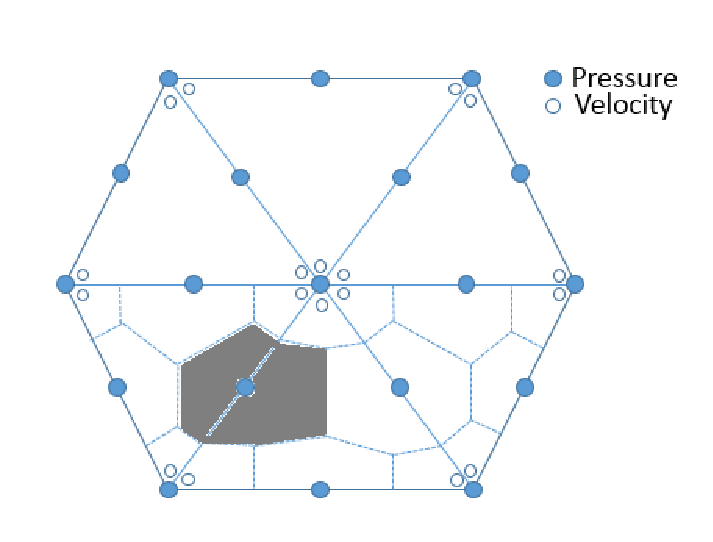
\includegraphics[width=.5\textwidth]{./Pics/P1DGP2.pdf}}
\caption{2D representation of \PN[1]{2} element pairs used in this work. Shaded areas denote control volumes across two contiguous elements. Blue and white circles represent pressure and velocity nodes, respectively.} 
\label{fig:fem_cv}
\end{figure}

\clearpage

%%%%
%%%%  FIGURE
%%%%
\begin{figure}[h]
\centering
\vbox{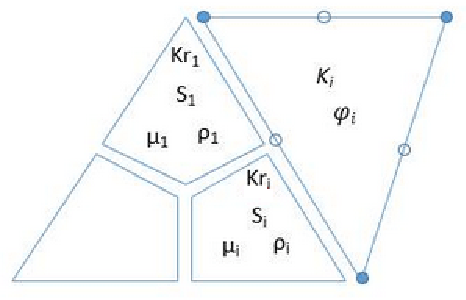
\includegraphics[width=.75\textwidth]{./Pics/element_n.pdf}}
\caption{This is a graphical representation of two different element types. Triangle {\it A} is a representation of the \PN[1]{2} element-pair, whereas triangle {\it B} represents the \PN[1]{1} element-pair. Porosity $\phi_{i}$, permeability {\bf K}$_{i}$, velocity and pressure are primarily represented in FE space whereas scalar fields (such as saturation, density, viscosity etc) are represented in CV space.}
\label{fig:fem_elem}
\end{figure}
\clearpage

%%%%
%%%%  FIGURE 
%%%%
\begin{figure}[h]
\centering
\vbox{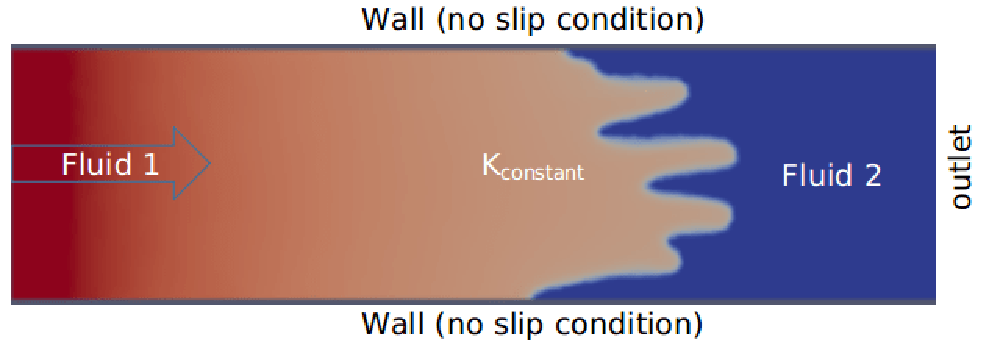
\includegraphics[width=0.75\textwidth]{./Pics/phase_vol_frac_uni_perm_1.pdf}}
\caption{Schematics of formation of flow instabilities during injection of a pure low viscosity fluid (red) into a domain saturated with a second fluid (dark blue). The ratio of viscosity between the two fluids is 5. In this case, the initially piston shape front collapses leading to the formation of several fingers.}
\label{fig:simple_case}
\end{figure}
\clearpage


%%%%
%%%%  FIGURE 
%%%%
\begin{figure}[ht] 
\vbox{
\hbox{\hspace{-0.3cm}
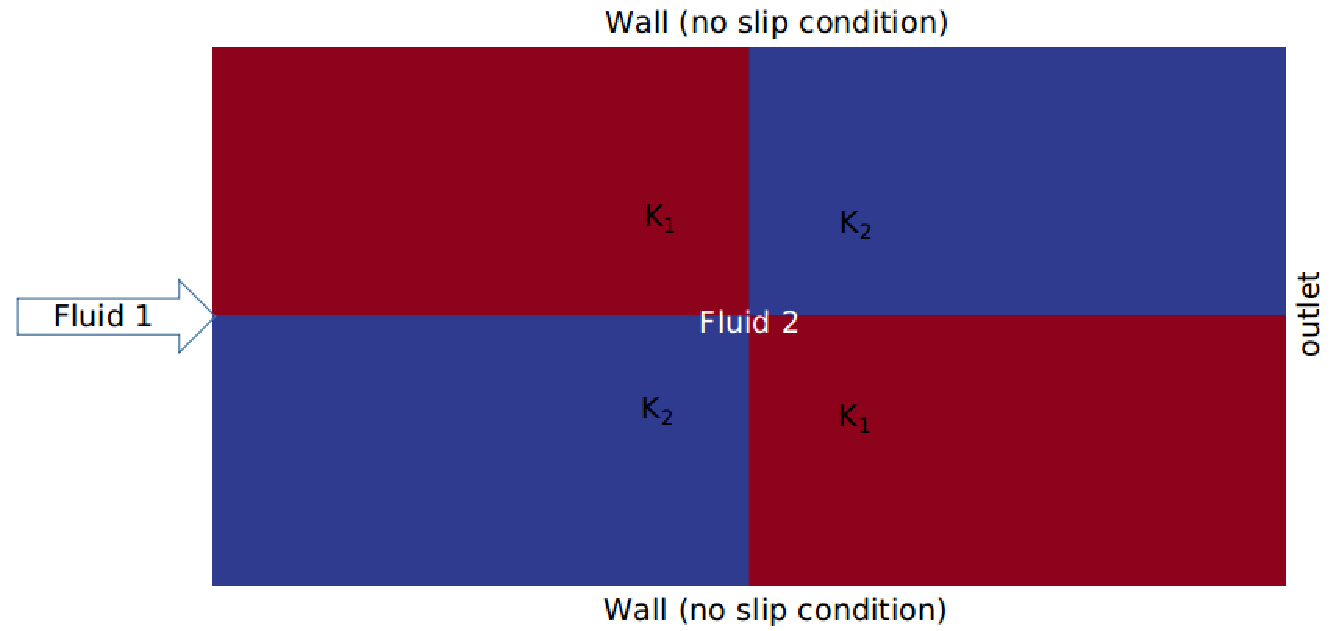
\includegraphics[width=.8\textwidth]{./Pics1/2b2_wi_fine/2b2_whole_in_fine_perm_1.pdf} 
}
\vspace{0.0cm}
\hbox{\hspace{3.5cm} (a) map of permeabilities ($\mathbf{K}$)
}
\vspace{0.25cm}
\hbox{\hspace{1.5cm}
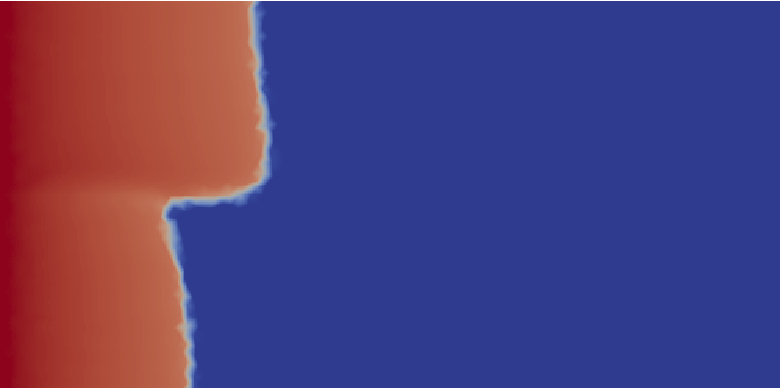
\includegraphics[width=.85\textwidth]{./Pics1/2b2_wi_fine/2b2_whole_in_fine_250_2.pdf}
}
\vspace{0.0cm}
\hbox{\hspace{4.5cm} (b) flow at t=250 
}
\vspace{0.25cm}
\hbox{\hspace{1.5cm}
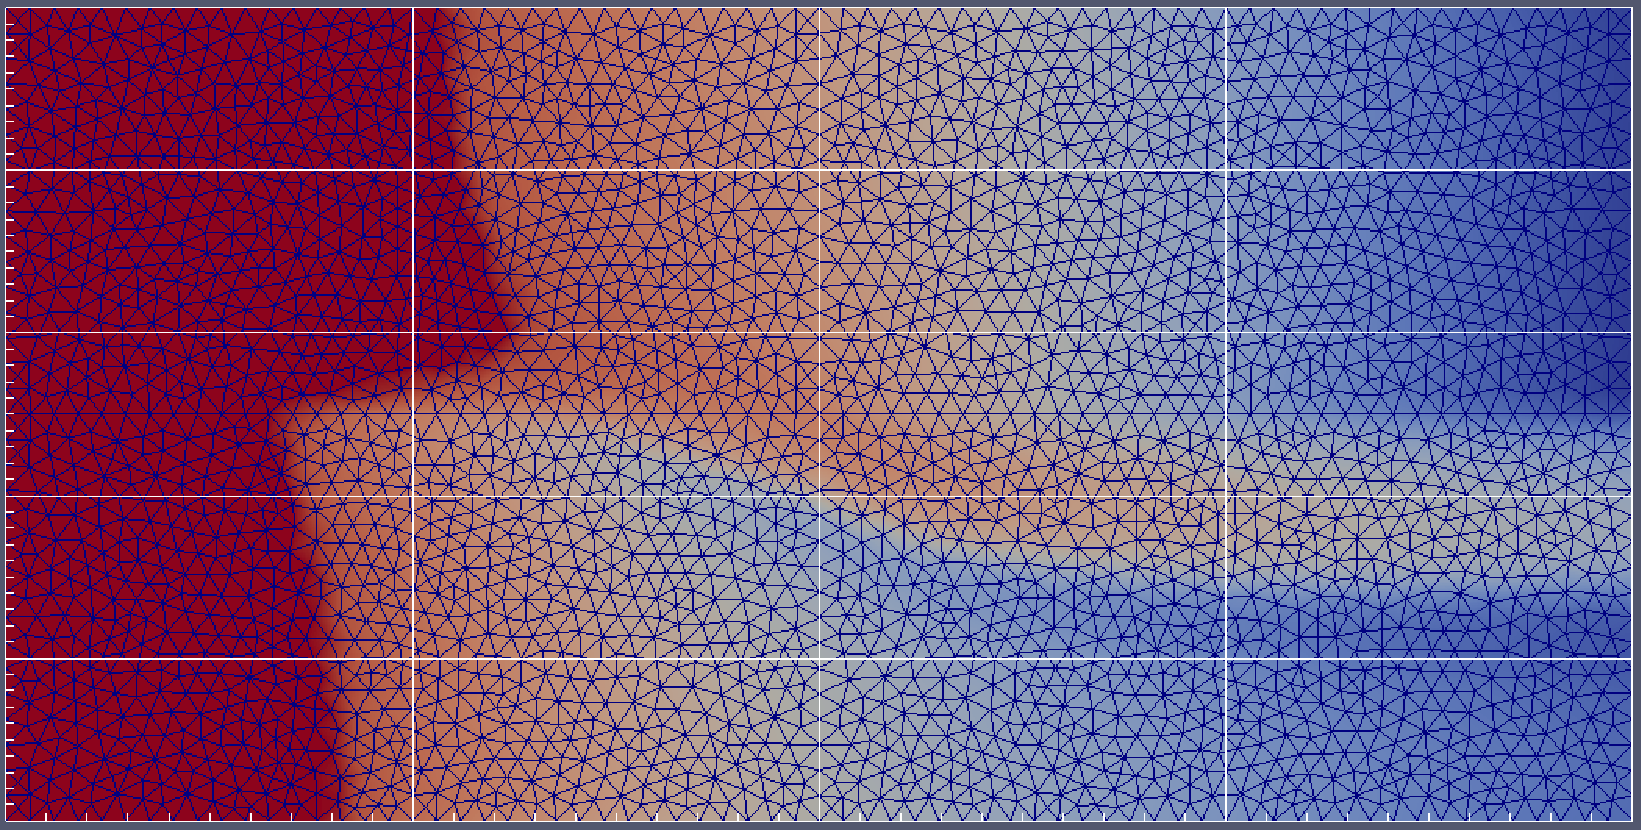
\includegraphics[width=.65\textwidth]{./Pics1/2b2_wi_fine/2b2_whole_in_fine_3000_2.pdf}
}
\vspace{0.0cm}
\hbox{\hspace{4.0cm} (c) flow at t=3000   
}}     
\caption{Model validation of fluid displacement in heterogeneous porous media ({\it VR}=1): (a) the domain is divided into four subdomains with prescribed synthetic permeability, $\mathbf{K}_{1}=1$ and $\mathbf{K}_{2}=2.5$; (b-c) snapshots of saturation (displacing fluid) field at t=$25$s and t=$300$ sec. The domain is discretised with $5960$ \PN[1]{2} elements. }
\label{fem_cv_represent_a}
\end{figure}
\clearpage



%%%%
%%%%  FIGURE
%%%%
\begin{landscape}
\begin{figure}[ht] 
\vbox{\vspace{-1cm}
\hbox{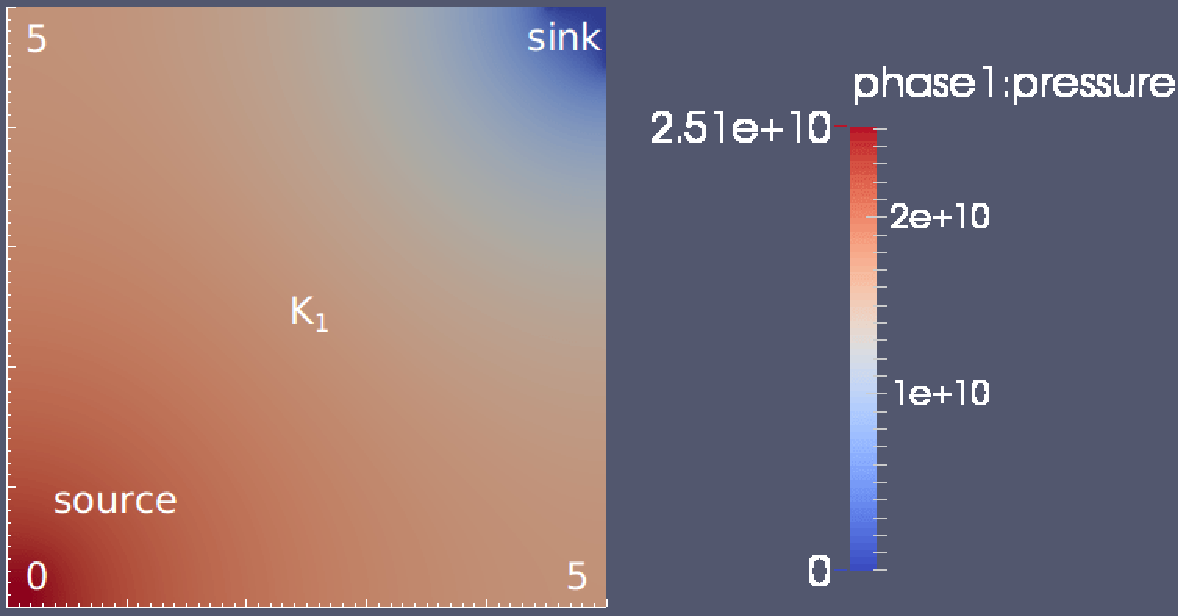
\includegraphics[width=.7\textwidth]{./Pics1/Saffman_homogeneous_MR3/saffman_homo_fixed_2.pdf}
      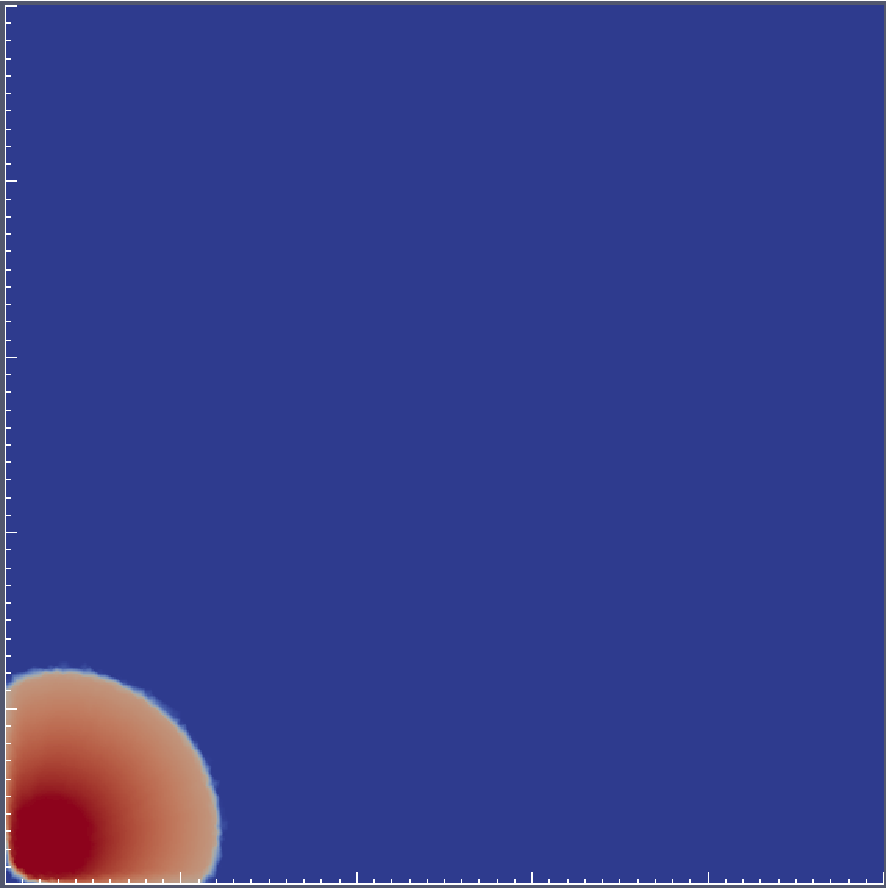
\includegraphics[width=.37\textwidth]{./Pics1/Saffman_homogeneous_MR3/saffman_homo_fixed_250.pdf}
      \includegraphics[width=.37\textwidth]{./Pics1/Saffman_homogeneous_MR3/saffman_homo_fixed_1000.pdf}}
\vspace{0.cm}
\hbox{\hspace{2.5cm} (a) pressure at t=0s \hspace{5.cm} (b) t=0.87s \hspace{2.75cm} (c) t=3.54s}
\vspace{0.5cm}
\hbox{
      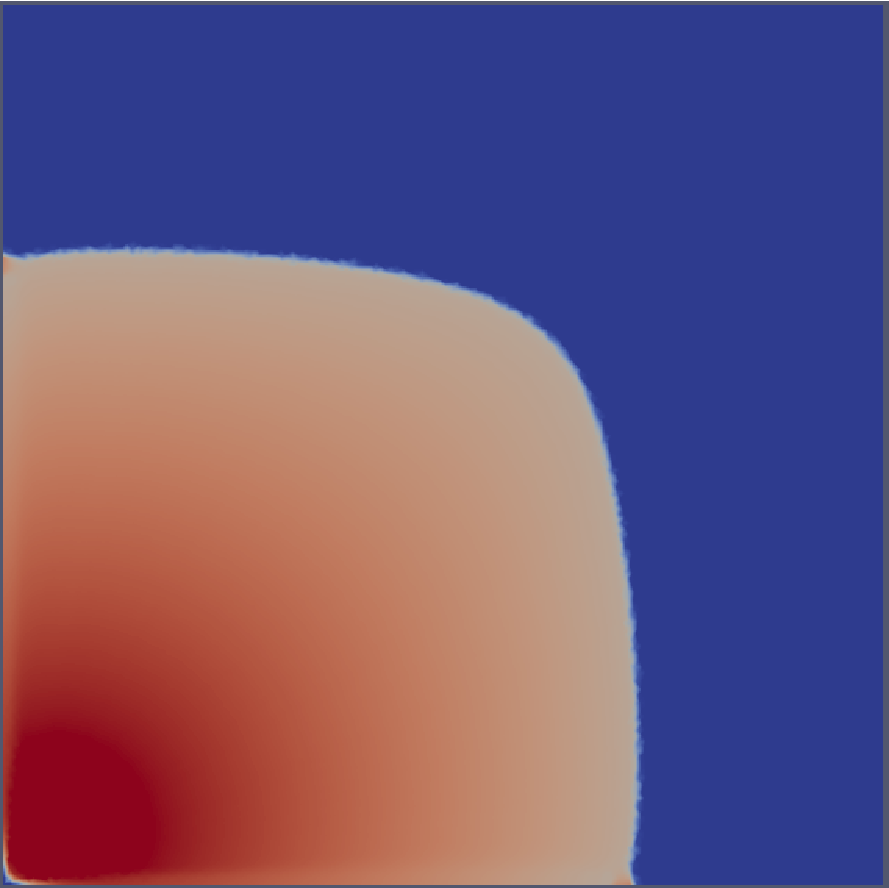
\includegraphics[width=.375\textwidth]{./Pics1/Saffman_homogeneous_MR3/saffman_homo_fixed_2500.pdf}
      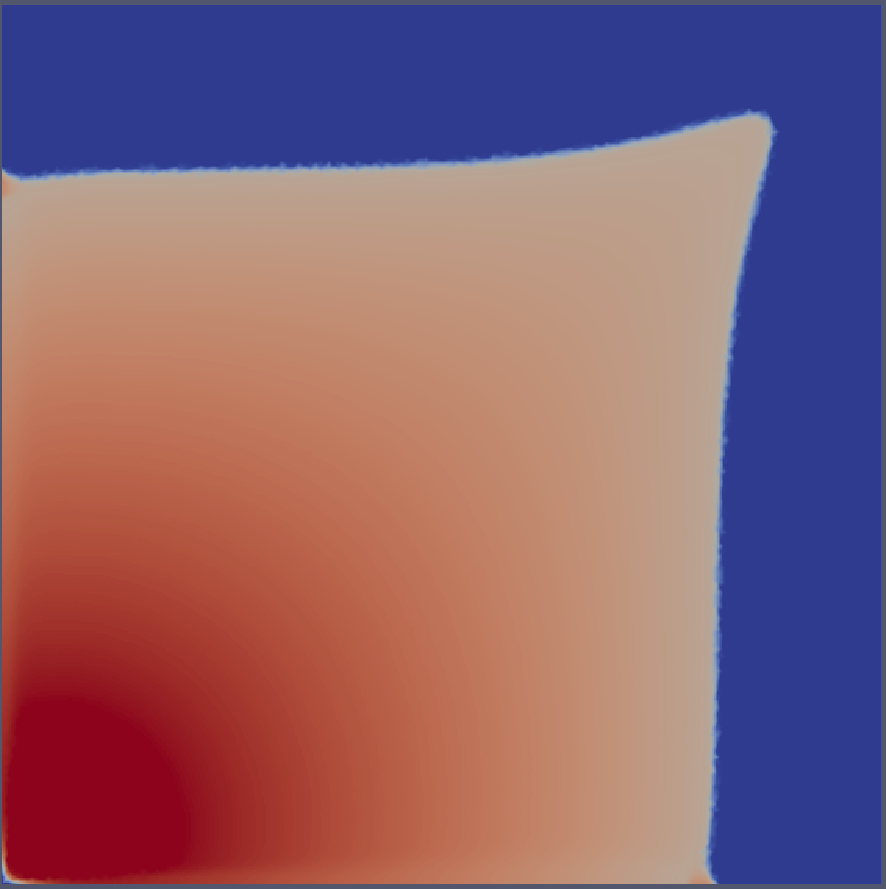
\includegraphics[width=.375\textwidth]{./Pics1/Saffman_homogeneous_MR3/saffman_homo_fixed_3500.pdf} 
      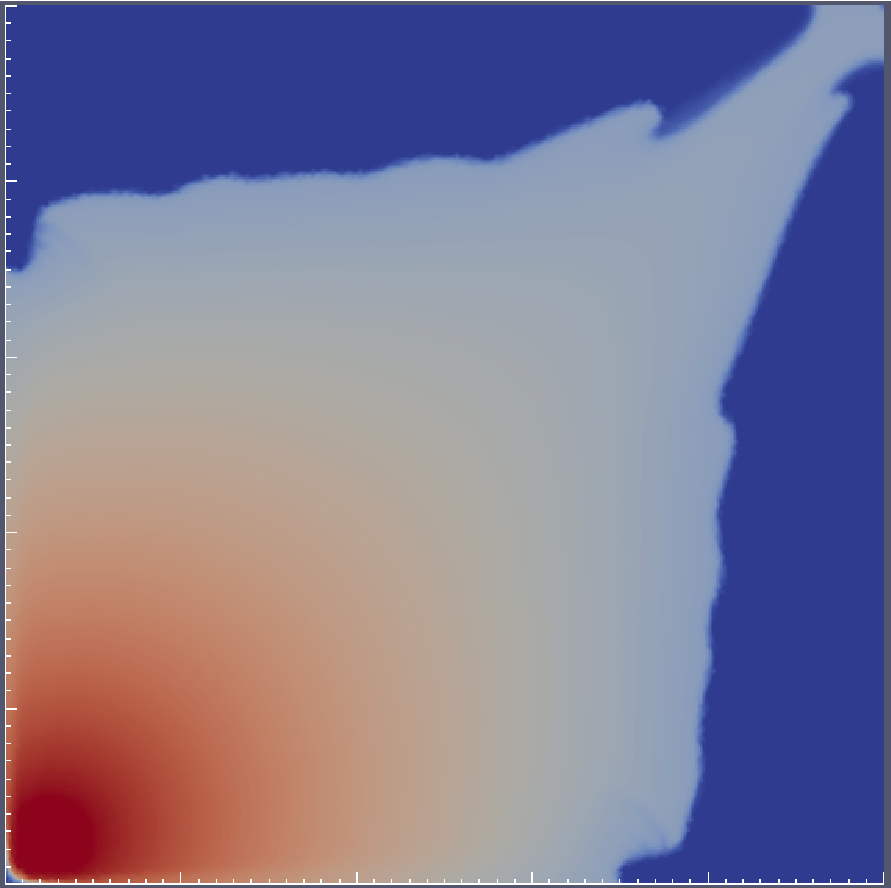
\includegraphics[width=.65\textwidth]{./Pics1/Saffman_homogeneous_MR3/saffman_homo_fixed_end.pdf}}
\vspace{0.cm}
\hbox{ \hspace{1.cm} (d) t=8.86s \hspace{3.0cm} (e) t=12.41s   \hspace{4.0cm} (f) t=17.95s}
\vspace{0.cm}
}   
\caption{Simulated flow in a Hele-Shaw cell ({\it VR}=3): (a) initial pressure profile $\left(\text{in g.cm}^{-1}\text{.s}^{-2}\right)$ with source and sink regions are explicitly shown along with dimensions (in cm); (b-f) snapshots of wetting phase saturation showing flow profile as the simulation evolves. The domain contains $47500$ \PN[1]{2} triangular elements.}
\label{fig:homoheleshaw_VN3}
\end{figure}
\end{landscape}
\clearpage



%%%%
%%%%  FIGURE
%%%%
\begin{landscape}
\begin{figure}[ht] 
\vbox{\vspace{-1cm}
\hbox{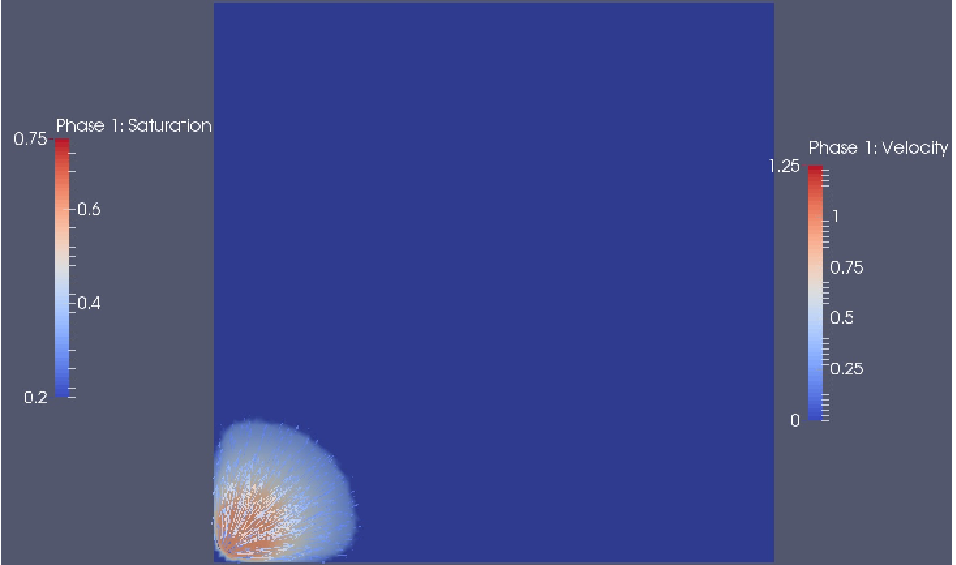
\includegraphics[width=.9\textwidth, height=0.5\textwidth]{./Pics1/Saffman_homogeneous_VR10/ST_Homog_VR10_D201c.pdf}
\hspace{0.5cm}      
      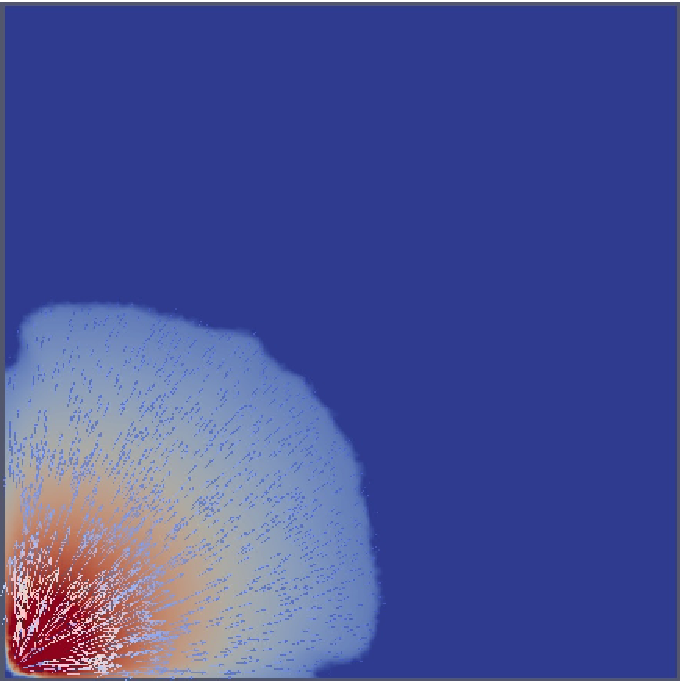
\includegraphics[width=.5\textwidth]{./Pics1/Saffman_homogeneous_VR10/ST_Homog_VR10_D1001c.pdf}}
\vspace{0.cm}
\hbox{\hspace{5.cm} (a) t=0.66s \hspace{8.cm} (b) t=3.43s }
\vspace{0.5cm}
\hbox{
      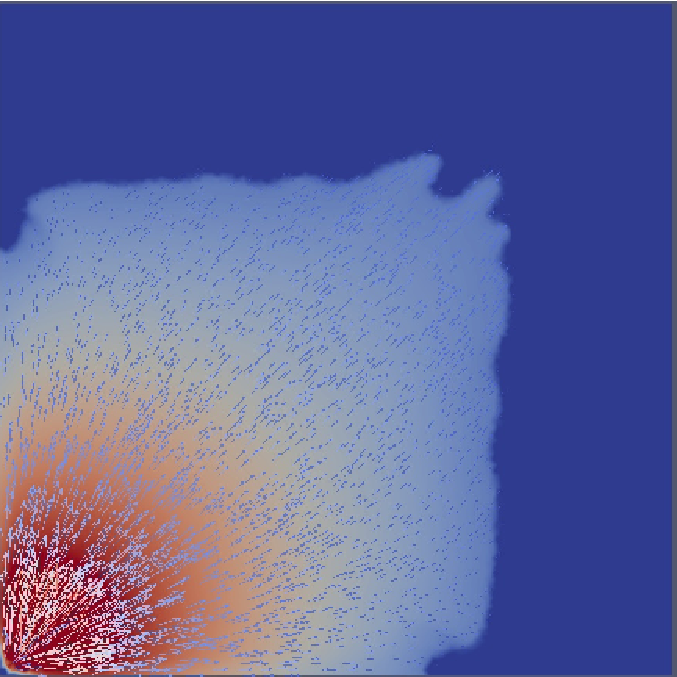
\includegraphics[width=.5\textwidth]{./Pics1/Saffman_homogeneous_VR10/ST_Homog_VR10_D2001c}
      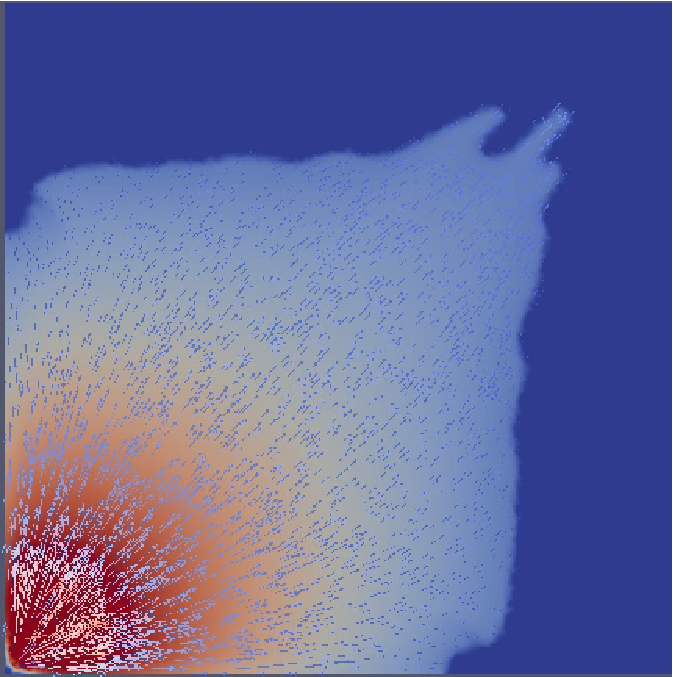
\includegraphics[width=.5\textwidth]{./Pics1/Saffman_homogeneous_VR10/ST_Homog_VR10_D2201c}
      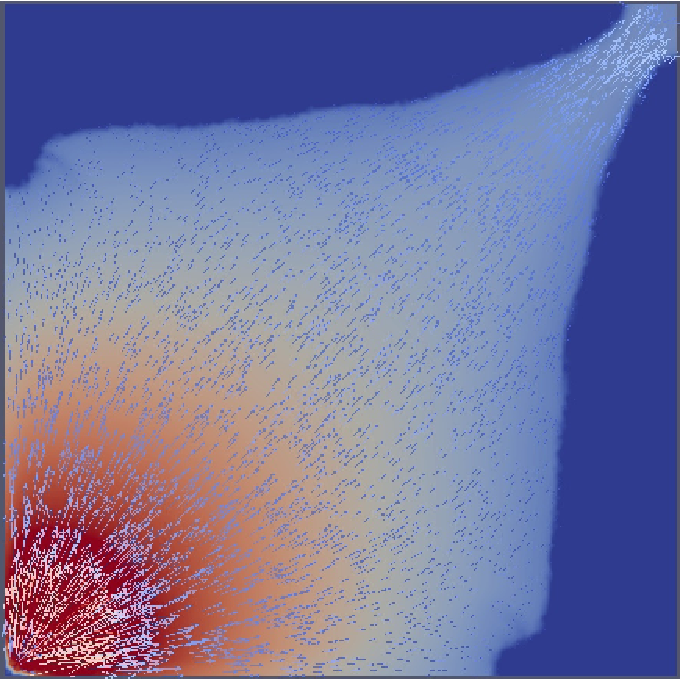
\includegraphics[width=.5\textwidth]{./Pics1/Saffman_homogeneous_VR10/ST_Homog_VR10_D3001c}}
\vspace{0.cm}
\hbox{ \hspace{2.cm} (c) t=6.92s \hspace{4.5cm} (d) t=7.61s \hspace{4.5cm} (e)t=10.00s}
\vspace{0.cm}
}   
\caption{Simulated flow in a Hele-Shaw cell ({\it VR}=10): snapshots of overlapped wetting phase saturation and velocity vectors showing flow profile as the simulation evolves. The domain contains $26313$ \PN[1]{2} triangular elements.}
\label{fig:homoheleshaw_VN10}
\end{figure}
\end{landscape}
\clearpage

%%%%
%%%%  FIGURE
%%%%
\begin{landscape}
\begin{figure}[ht] 
\vbox{\vspace{-1cm}
\hbox{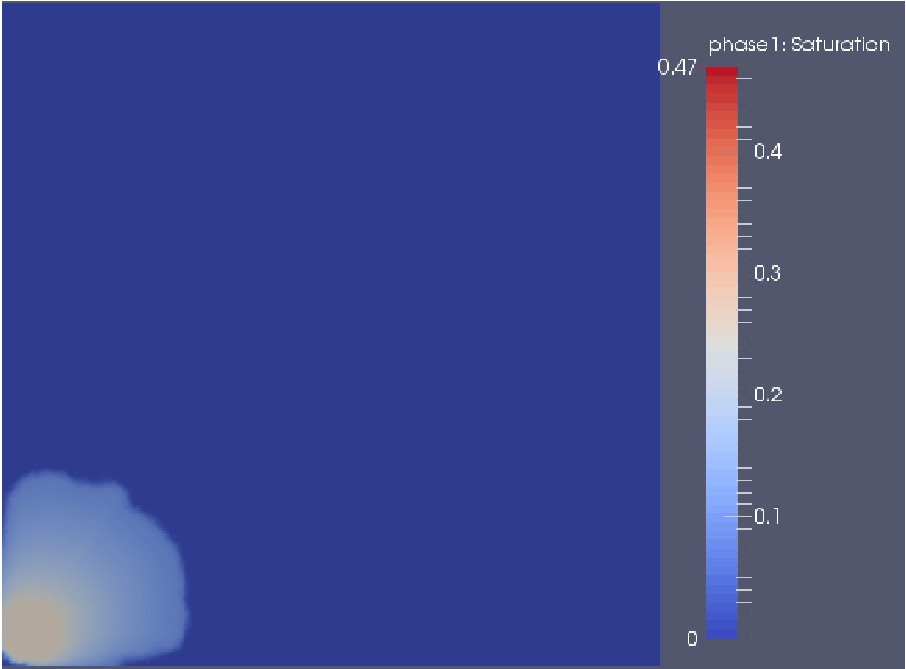
\includegraphics[width=.9\textwidth, height=0.5\textwidth]{./Pics1/Saffman_homogeneous_VR150/ST_Homog_VR150_D300b}
\hspace{0.5cm}      
      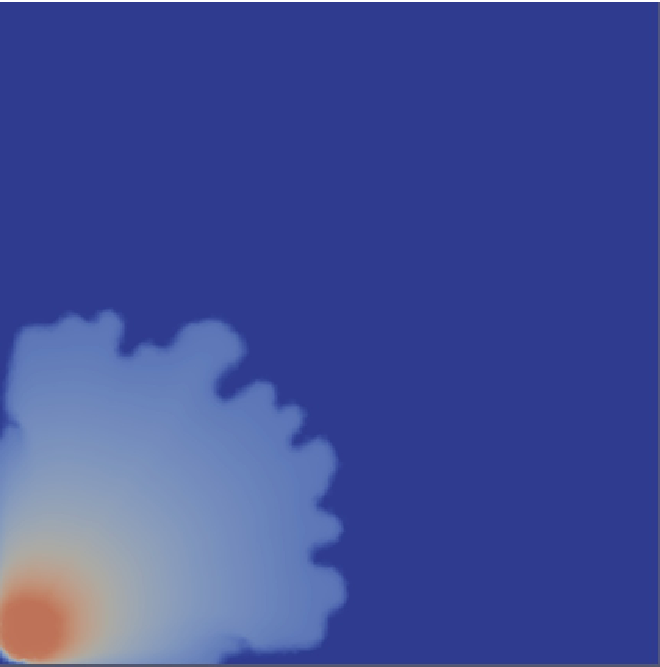
\includegraphics[width=.5\textwidth]{./Pics1/Saffman_homogeneous_VR150/ST_Homog_VR150_D1600b}}
\vspace{0.cm}
\hbox{\hspace{5.cm} (a) t=0.27s \hspace{8.cm} (b) t=0.94s }
\vspace{0.5cm}
\hbox{
      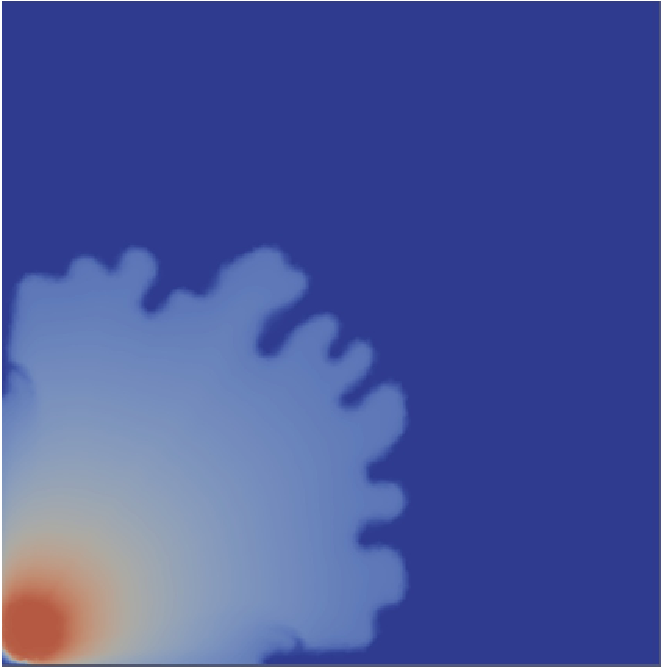
\includegraphics[width=.5\textwidth]{./Pics1/Saffman_homogeneous_VR150/ST_Homog_VR150_D2700b}
      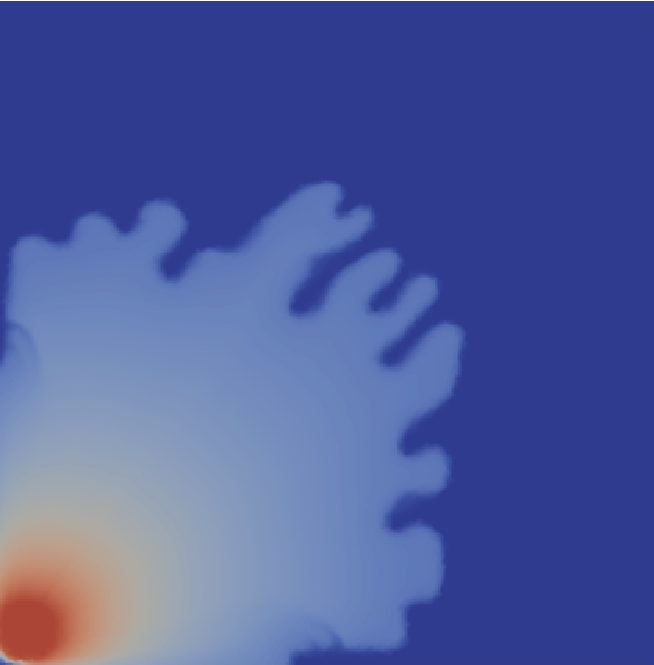
\includegraphics[width=.5\textwidth]{./Pics1/Saffman_homogeneous_VR150/ST_Homog_VR150_D4000b}
      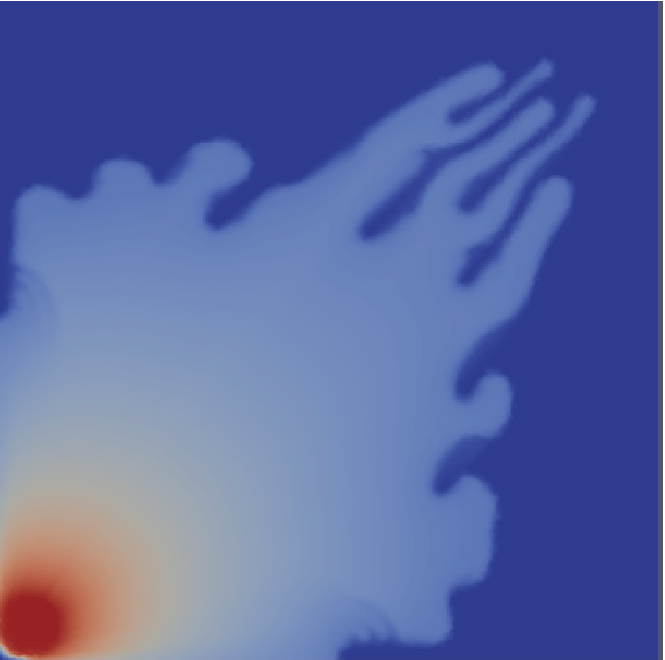
\includegraphics[width=.5\textwidth]{./Pics1/Saffman_homogeneous_VR150/ST_Homog_VR150_D7000b}}
\vspace{0.cm}
\hbox{ \hspace{2.cm} (c) t=1.32s \hspace{4.5cm} (d) t=1.70s \hspace{4.5cm} (e)t=2.31s}
\vspace{0.cm}
}   
\caption{Simulated flow in a Hele-Shaw cell ({\it VR}=150): snapshots of wetting phase saturation showing flow profile as the simulation evolves. The domain contains $26313$ \PN[1]{2} triangular elements.}
\label{fig:homoheleshaw_VN10}
\end{figure}
\end{landscape}
\clearpage


%%%%
%%%%  FIGURE
%%%%
\begin{landscape}
\begin{figure}[ht] 
\hbox{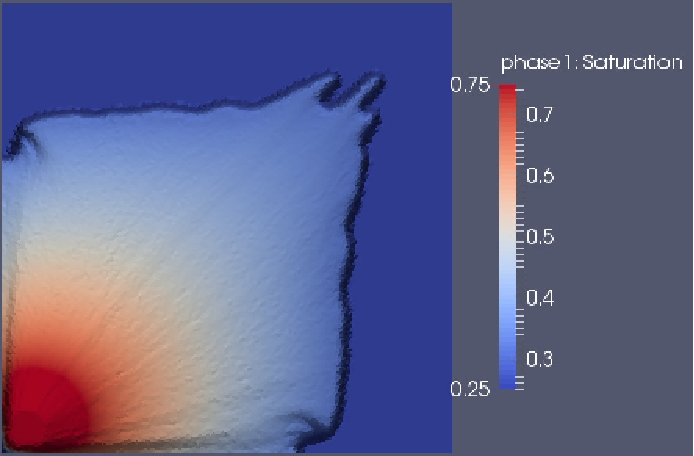
\includegraphics[width=.5\textwidth]{./Pics1/Saffman_homogeneous_VR10/ST_Homog_VR10_D2201_bbd}
       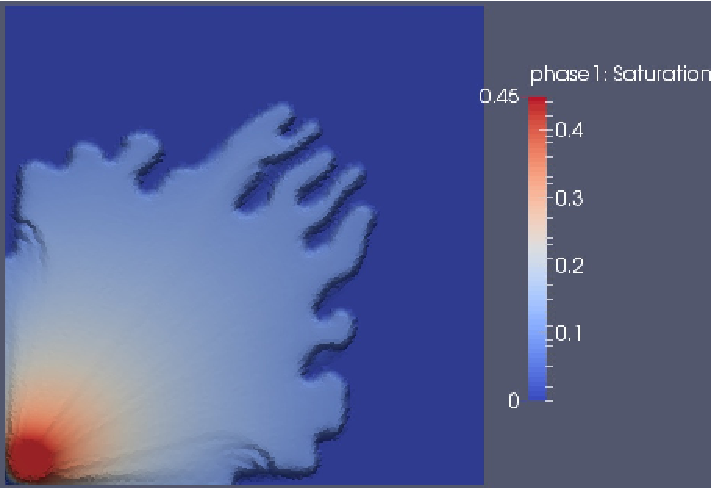
\includegraphics[width=.49\textwidth]{./Pics1/Saffman_homogeneous_VR150/ST_Homog_VR150_D5003_k2b}}
\caption{Simulated flow in Hele-Shaw cells performed with viscosity ratios of 10 (left, t=7.61s) and 150 (t=1.94s). Width of largest fingers are approximetely 0.70 and 0.90cm, which are in good agreement with values obtained from \citet{guan_2003}'s analytic solution. Domains of both simulations contain $26313$ \PN[1]{2} triangular elements.\red{(More pics to be added!!)}}
\label{fig:homoheleshaw_VN10_VN150}
\end{figure}
\end{landscape}



\begin{comment}

%%%%
%%%%  FIGURE
%%%%
\begin{landscape}
\begin{figure}[ht] 
\vbox{\vspace{-1cm}
\hbox{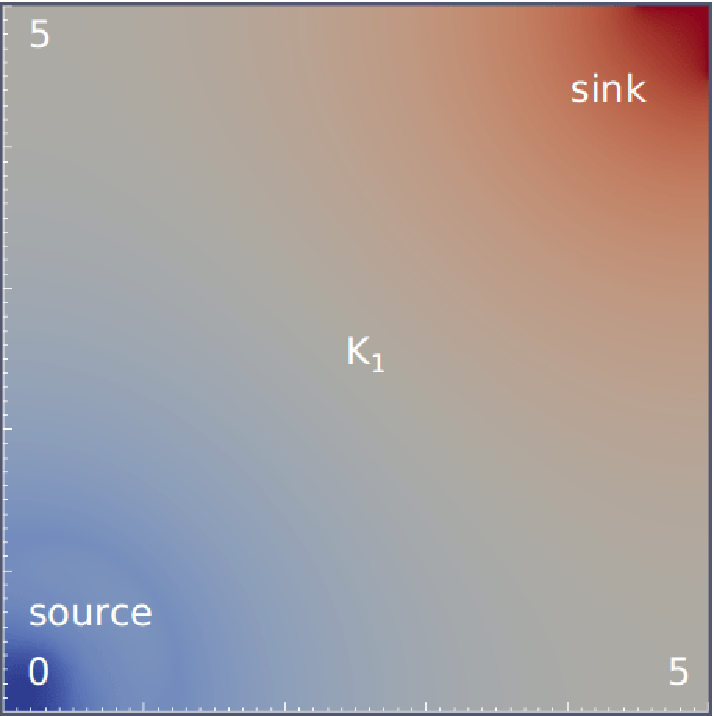
\includegraphics[width=.5\textwidth]{./Pics1/Saffman_homogeneous/saffman_homo_fixed_1.pdf}
      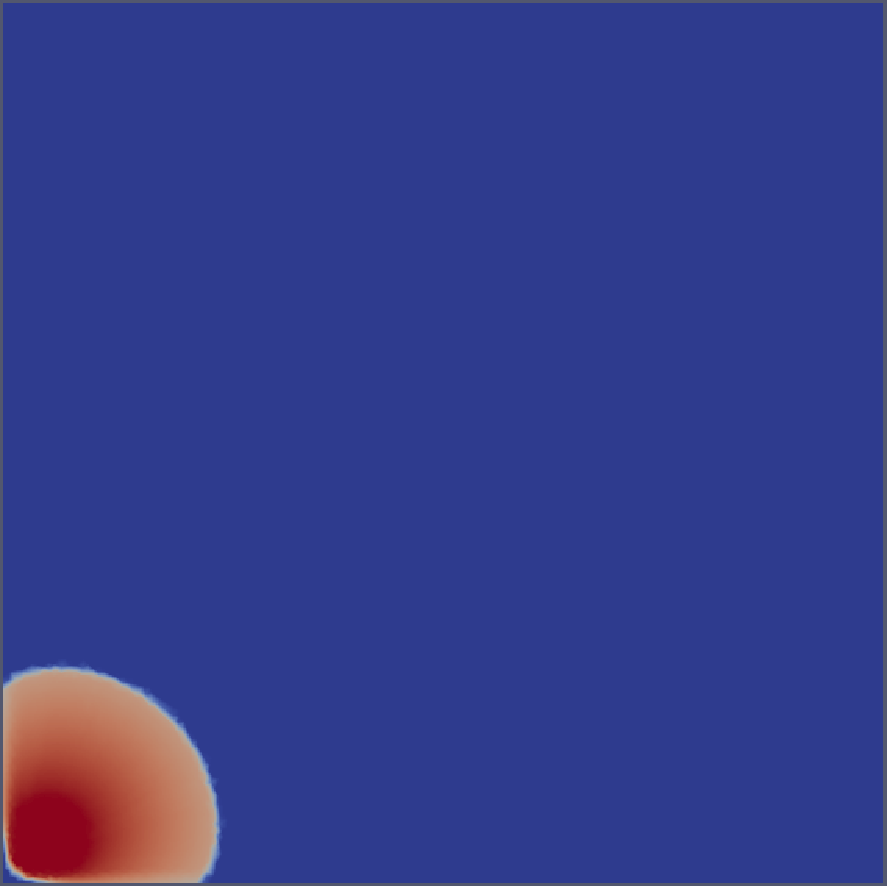
\includegraphics[width=.5\textwidth]{./Pics1/Saffman_homogeneous/saffman_homo_fixed_250_1.pdf}
      \includegraphics[width=.5\textwidth]{./Pics1/Saffman_homogeneous/saffman_homo_fixed_1000.pdf}}
\vspace{0.cm}
\hbox{\hspace{1.0cm} (a) pressure at t=0 \hspace{3.cm} (b) t=250\red{(???)} \hspace{3.0cm} (c) t=1000\red{(???)}}
\vspace{0.5cm}
\hbox{
      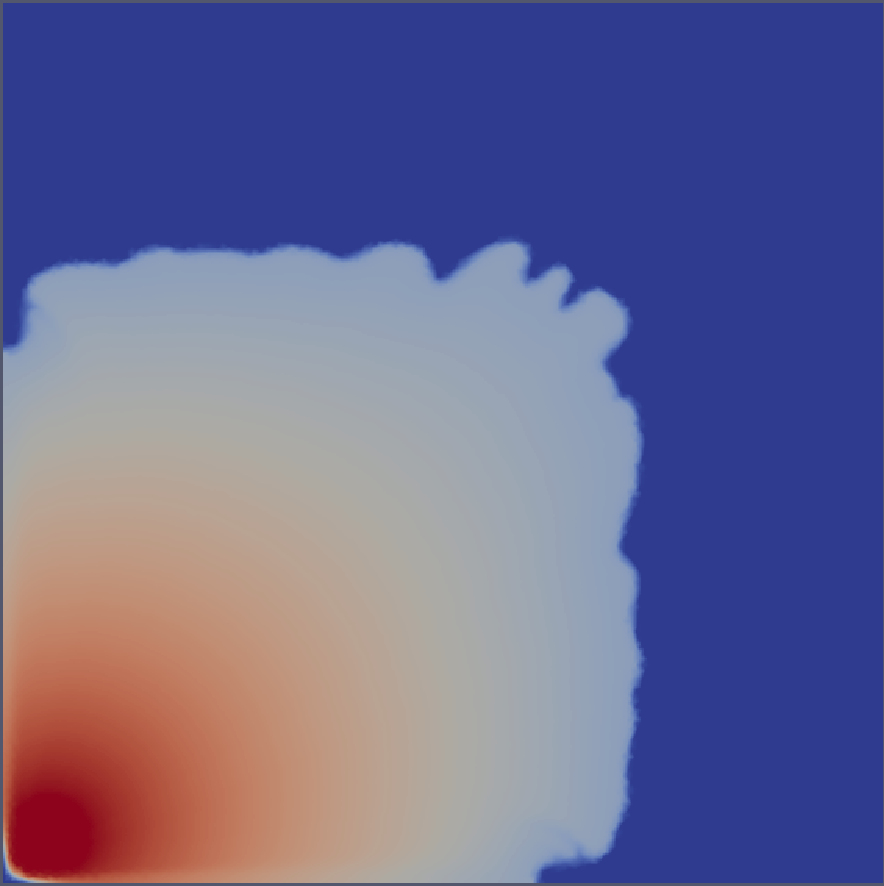
\includegraphics[width=.5\textwidth]{./Pics1/Saffman_homogeneous/saffman_homo_fixed_6000.pdf}
      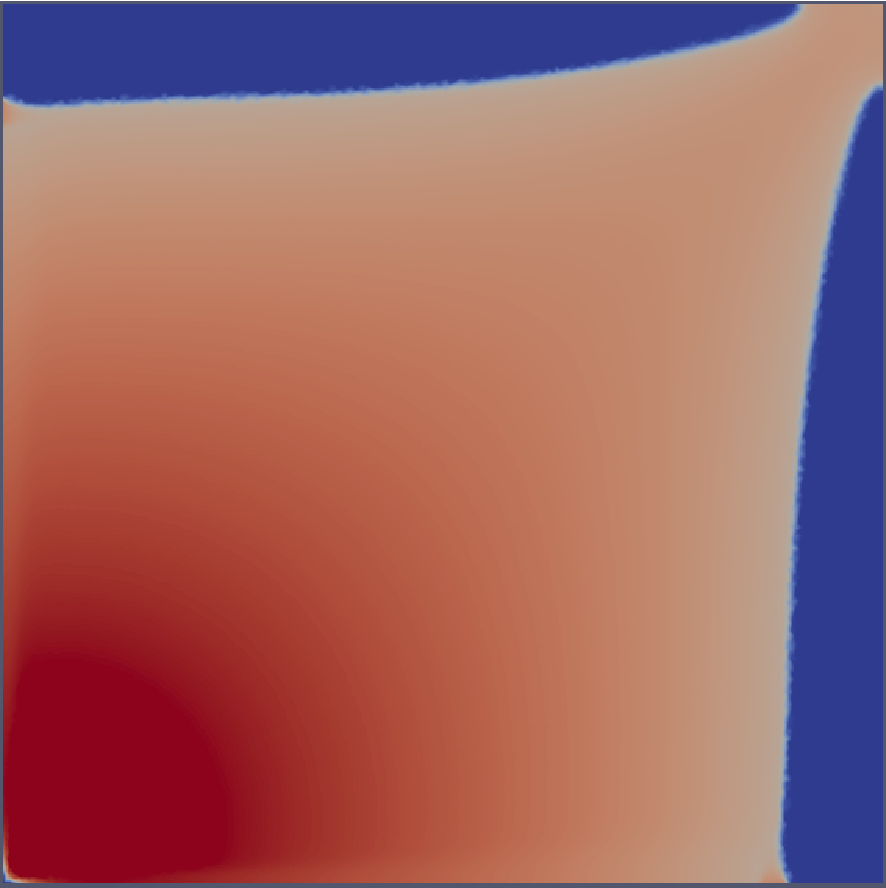
\includegraphics[width=.5\textwidth]{./Pics1/Saffman_homogeneous/saffman_homo_fixed_end_1.pdf}}
\vspace{0.cm}
\hbox{ \hspace{2.cm} (d) t=6000\red{(???)} \hspace{3.cm} (e) t=XXX\red{(???)}}
\vspace{0.cm}
}   
\caption{Simulated flow in a Hele-Shaw cell ({\it VR}=10): (a) pressure profile $\left(\text{in g.cm}^{-1}\text{.s}^{-2}\right)$ with source and sink regions explicitly shown along with dimensions (in cm); (b-e) snapshots of wetting phase saturation showing flow profile as the simulation evolves. The domain contains $47000$ \PN[1]{2} triangular elements. The pressure and saturation range of values are the same like the  case in fig.\ref{fig:homoheleshaw_VN3}.}
\label{fig:homoheleshaw_VN10}
\end{figure}
\end{landscape}
\clearpage
\end{comment}


%%%
%%% FIGURE XXXXXX
%%%
\begin{landscape}
  \begin{figure}[ht]
  \vbox{\vspace{-1cm}
      \hbox{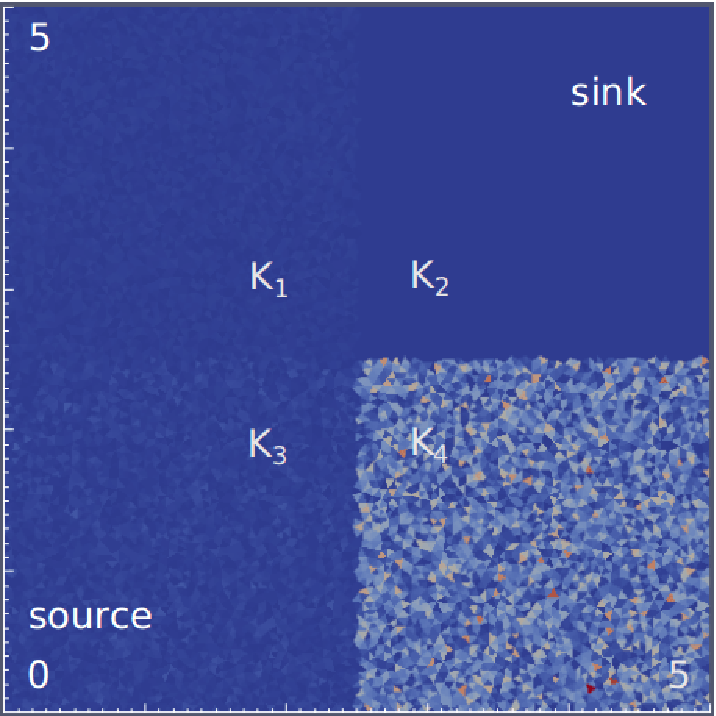
\includegraphics[width=.5\textwidth]{./Pics1/Saffman_heterogeneous/saffman_heter_fixed_1.pdf}
            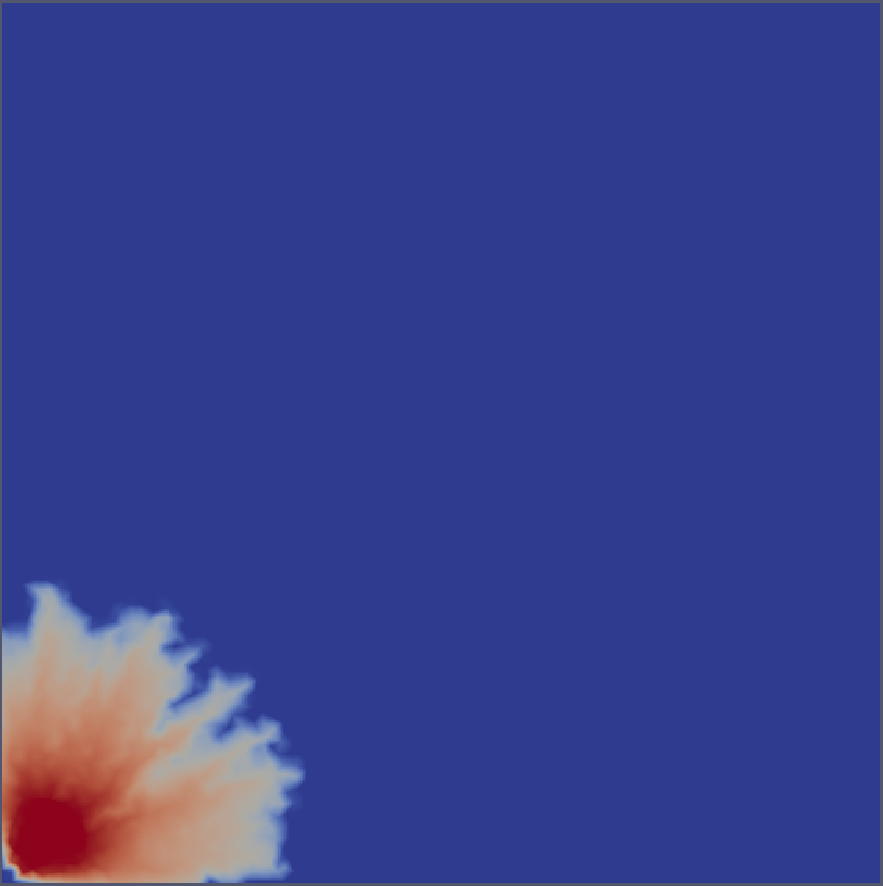
\includegraphics[width=.5\textwidth]{./Pics1/Saffman_heterogeneous/saffman_heter_fixed_500.pdf} 
            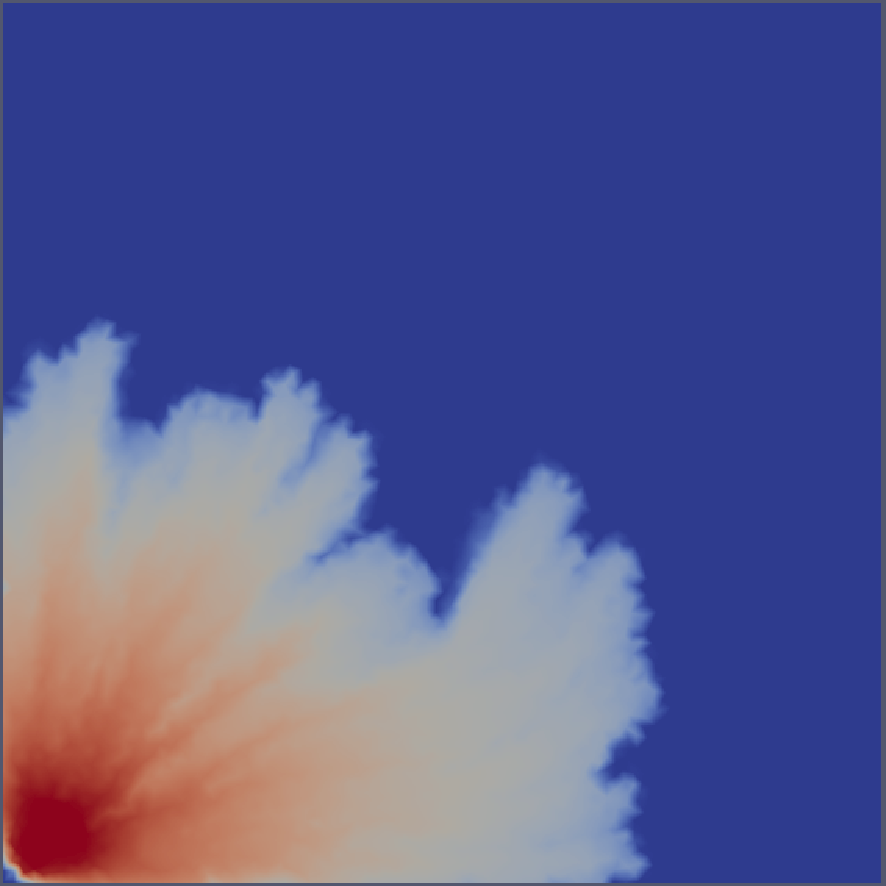
\includegraphics[width=.5\textwidth]{./Pics1/Saffman_heterogeneous/saffman_heter_fixed_2000.pdf} }
      \hbox{\hspace{1.0cm} (a) permeability map \hspace{3.cm} (b) t=0.75s \hspace{4.0cm} (c) t=8s}
      \vspace{0.5cm}
      \hbox{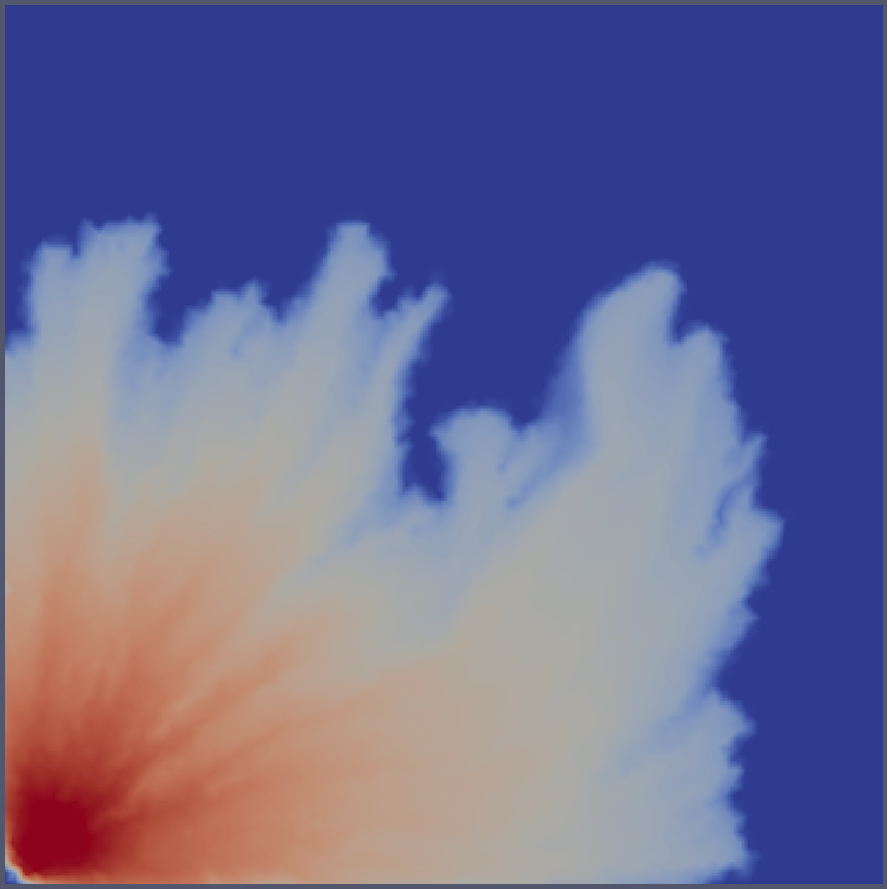
\includegraphics[width=.5\textwidth]{./Pics1/Saffman_heterogeneous/saffman_heter_fixed_3000.pdf}
            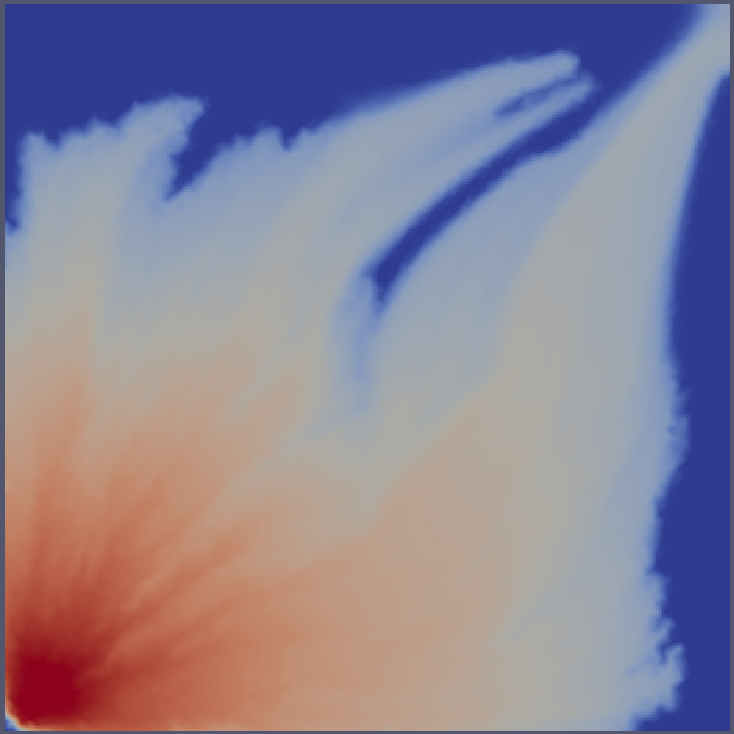
\includegraphics[width=.5\textwidth]{./Pics1/Saffman_heterogeneous/saffman_heter_fixed_6000.pdf}
            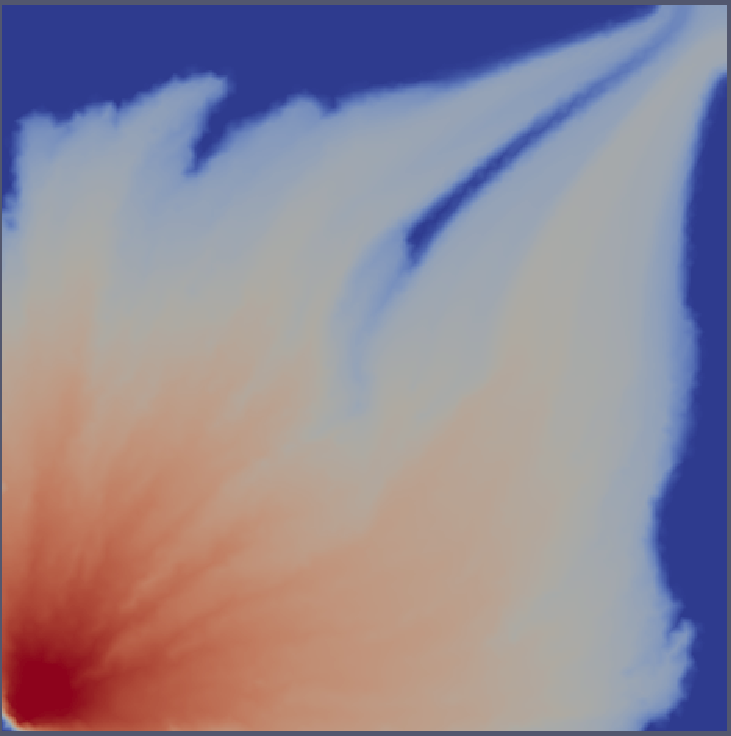
\includegraphics[width=.5\textwidth]{./Pics1/Saffman_heterogeneous/saffman_heter_fixed_24000.pdf} }
      \hbox{\hspace{2.5cm} (d) t=18s \hspace{5.cm} (e) t= \hspace{3.0cm} (f) t=24000 }}
\caption{Simulated flow in a modified Hele-Shaw cell with {\it VR}=10: (a) permeability distribution $\left(\text{10}^{-10}\le\mathbf{K}_{1}\le\text{5}\times\text{10}^{-10}\right.$, {\bf K}$_{2}$=10$^{-10}$, 10$^{-11}\le\mathbf{K}_{3}\le$ 5$\times$10$^{-10}$ and 10$^{-12}\le\mathbf{K}_{4}\le$ 5$\times$10$\left.^{-10}\text{ cm}^{2}\right)$; (b-f) snapshots of saturation profile during \red{XX} seconds of simulation. The domain contains \red{XX} \PN[1]{2} element-pairs.}
\label{fig:HeleShawHeter_VR10}
\end{figure}
\end{landscape}
\clearpage



%%%%
%%%%  FIGURE
%%%%
\begin{landscape}
\begin{figure}[ht] 
\vbox{
\hbox{\hspace{4.0cm}
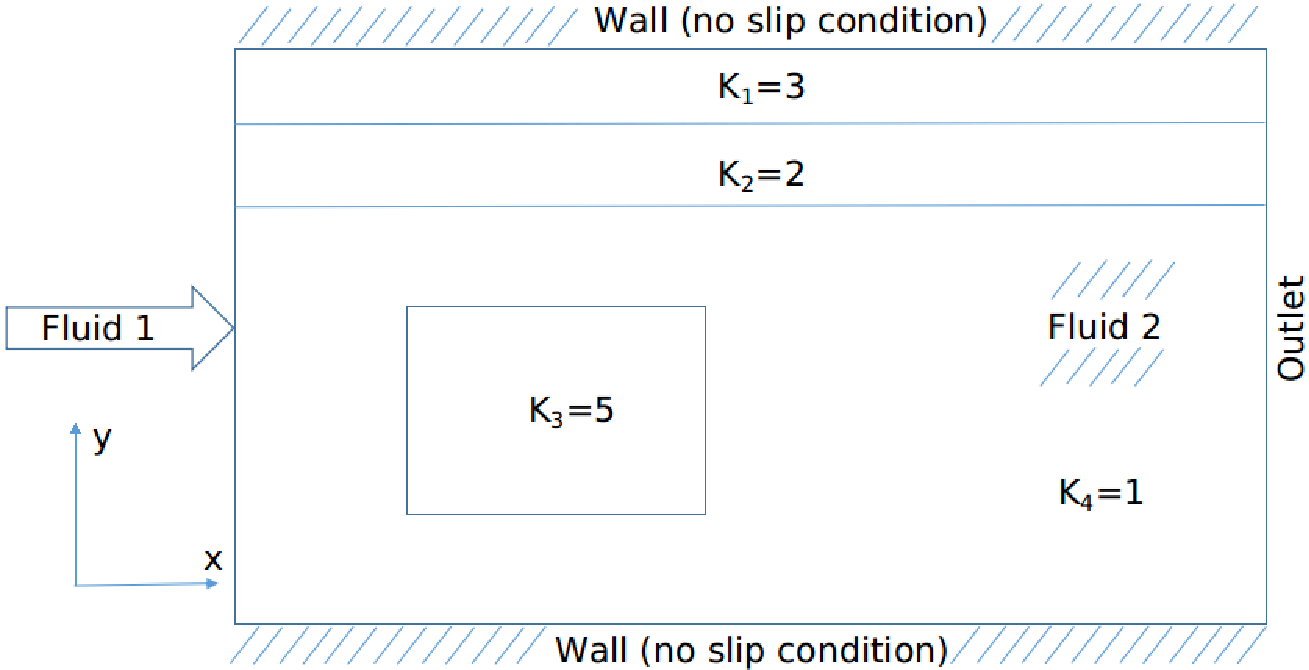
\includegraphics[width=.75\textwidth]{./Pics/map_of_boundaries.pdf} 
}
\vspace{0.0cm}
\hbox{\hspace{6.5cm} (a) map of permeabilties K   
}
\vspace{0.25cm}
\hbox{\hspace{4.0cm}
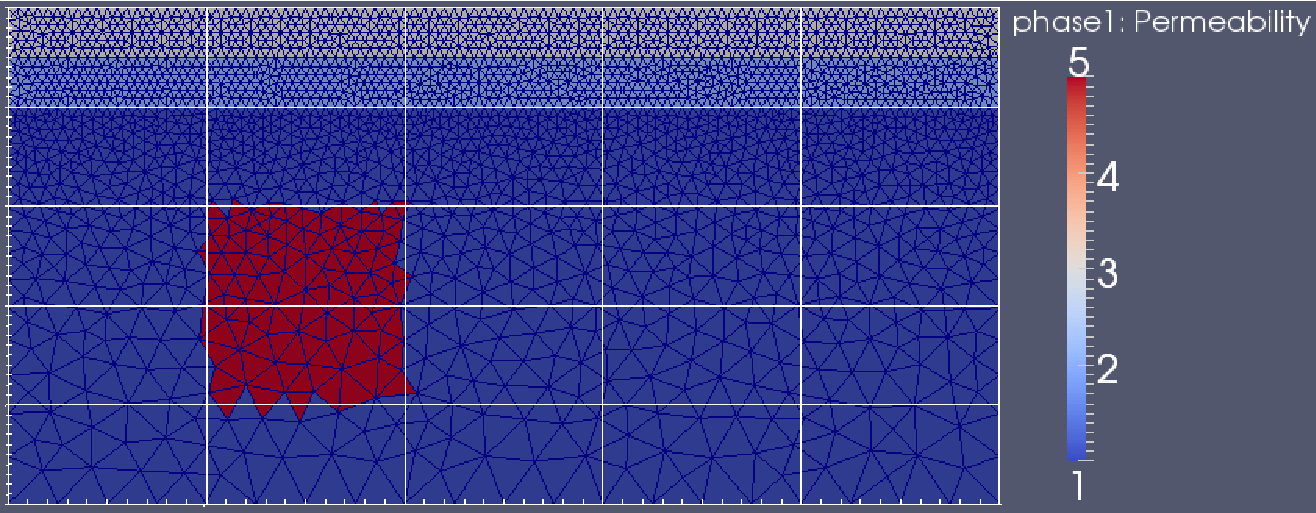
\includegraphics[width=.9\textwidth]{./Pics/map_of_boundaries_1.pdf}
}
\vspace{0.0cm}
\hbox{\hspace{9cm} (b)      
}
}     
\caption{Figure (a) describes the initial and boundary conditions as these are applied in this set of simulations. Below (b) there is a comparison between the unstructured and fixed mesh and the unstructured and adaptive mesh. During the implementation of fixed mesh initially there $4606$ elements while for the adaptive mesh there are $606$ while the majority of them is on the interface between between the two fluids. }
\label{fig:testcase_heter_domain}
\end{figure}
\end{landscape}
\clearpage



%%%%
%%%%  FIGURE
%%%%
\begin{landscape}
\begin{figure}[ht] 
\vbox{
\hbox{\hspace{3.5cm}
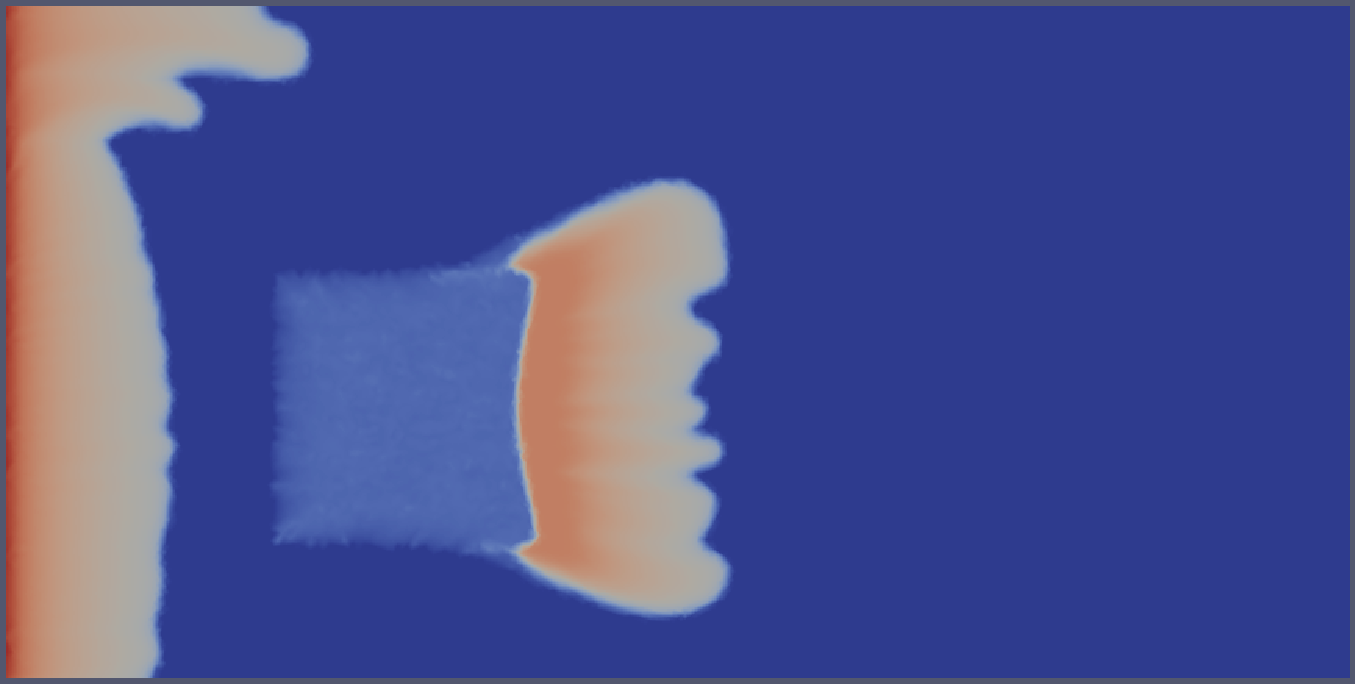
\includegraphics[width=.65\textwidth]{./Pics1/mr10_5regions_fixed/5regions_fixed_250.pdf} 
}
\vspace{0.0cm}
\hbox{\hspace{6.5cm} (a) flow at t=250 (fixed mesh)  
}
\vspace{0.25cm}
\hbox{\hspace{3.5cm}
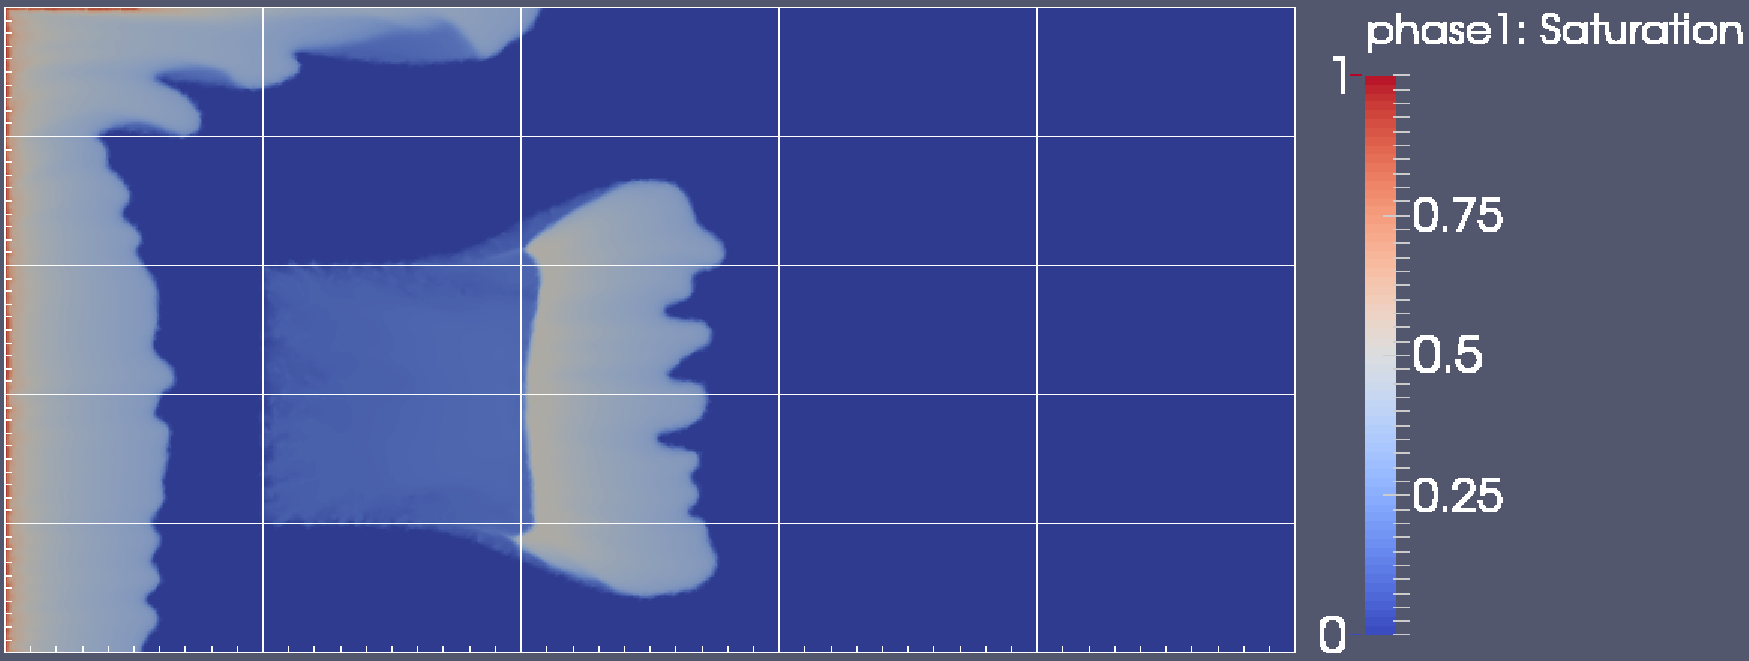
\includegraphics[width=.9\textwidth]{./Pics1/mr10_5regions_adapt/5regions_adapt_250_1.pdf}
}
\vspace{0.0cm}
\hbox{\hspace{6.5cm} (b) flow at t=250 (adaptive mesh)    
}
}     
\caption{For $t=0.125$s, $2$ test-cases under the VR=$10$ and under fixed (top) and adaptive(bottom) mesh are compared. There is a significant difference on the main front (left hand side of the domain) and the number of finger that appear.}
\label{fig:2testcase_a}
\end{figure}
\end{landscape}
\clearpage


%%%%
%%%%  FIGURE
%%%%
\begin{landscape}
\begin{figure}[ht] 
\vbox{
\hbox{\hspace{3.5cm}
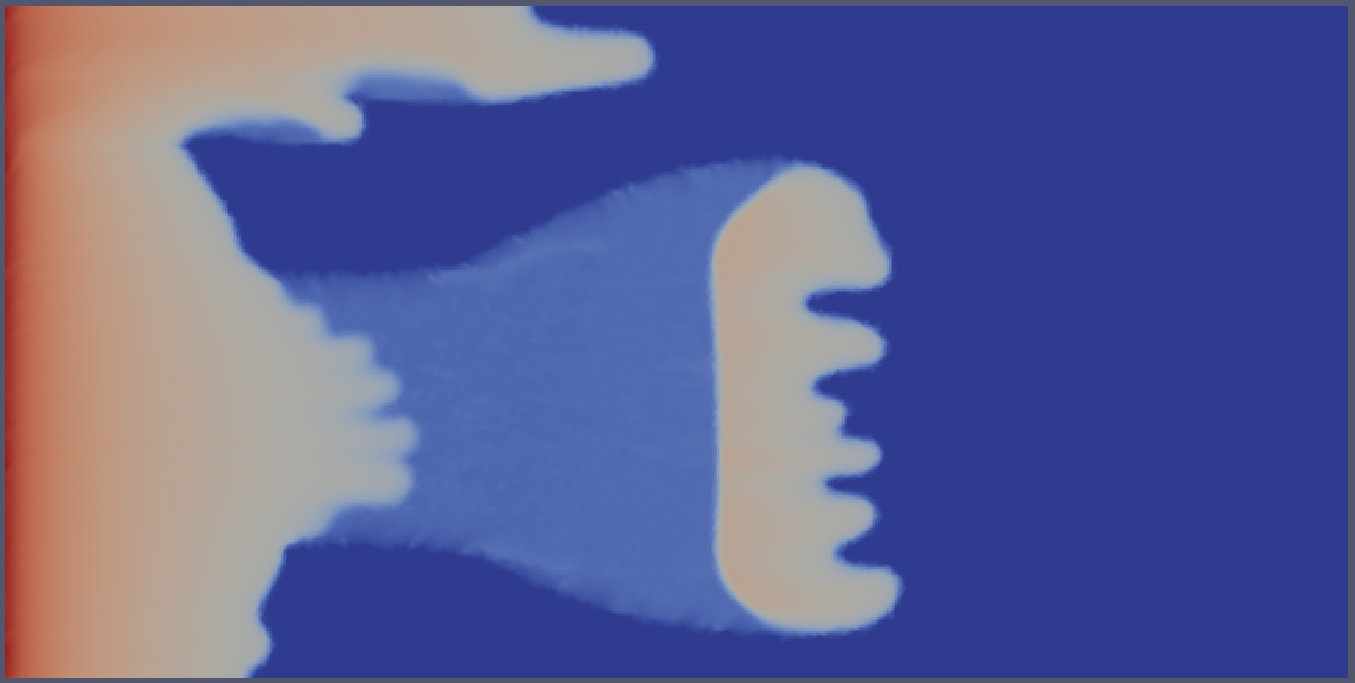
\includegraphics[width=.65\textwidth]{./Pics1/mr10_5regions_fixed/5regions_fixed_500.pdf} 
}
\vspace{0.0cm}
\hbox{\hspace{6.5cm} (a) flow at t=500 (fixed mesh)   
}
\vspace{0.25cm}
\hbox{\hspace{3.5cm}
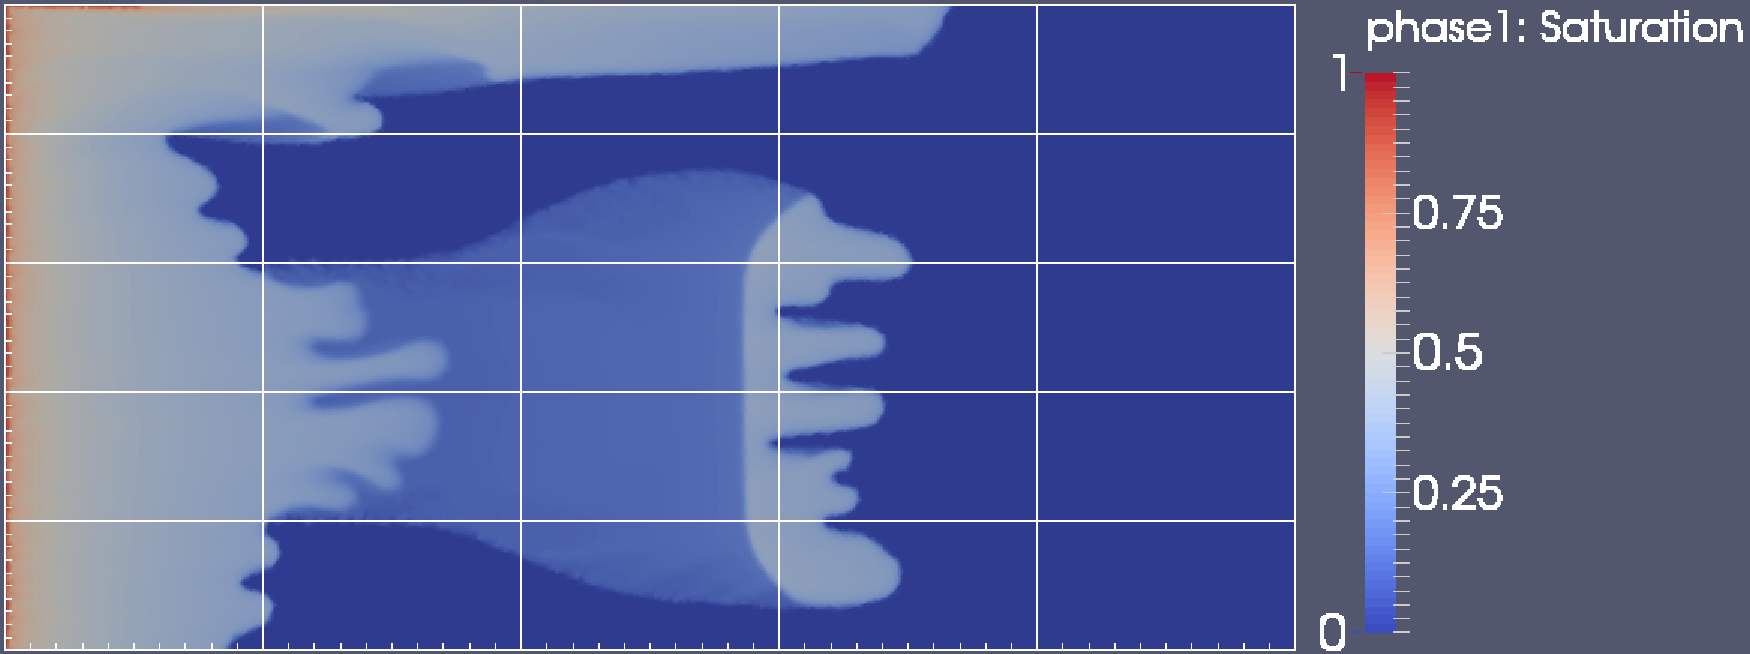
\includegraphics[width=.9\textwidth]{./Pics1/mr10_5regions_adapt/5regions_adapt_500_1.pdf}
}
\vspace{0.0cm}
\hbox{\hspace{6.5cm} (b) flow at t=500 (adaptive mesh)     
}
}     
\caption{At $t=0.25$s ($t=500$, timestemp) cross flow is taking place at the upper part of the formation. The fingers start to becoming more proufound as can been seen at the bottom.}
\label{fig:2testcase_b}
\end{figure}
\end{landscape}
\clearpage



%%%%
%%%%  FIGURE
%%%%
\begin{landscape}
\begin{figure}[ht] 
\vbox{
\hbox{\hspace{3.5cm}
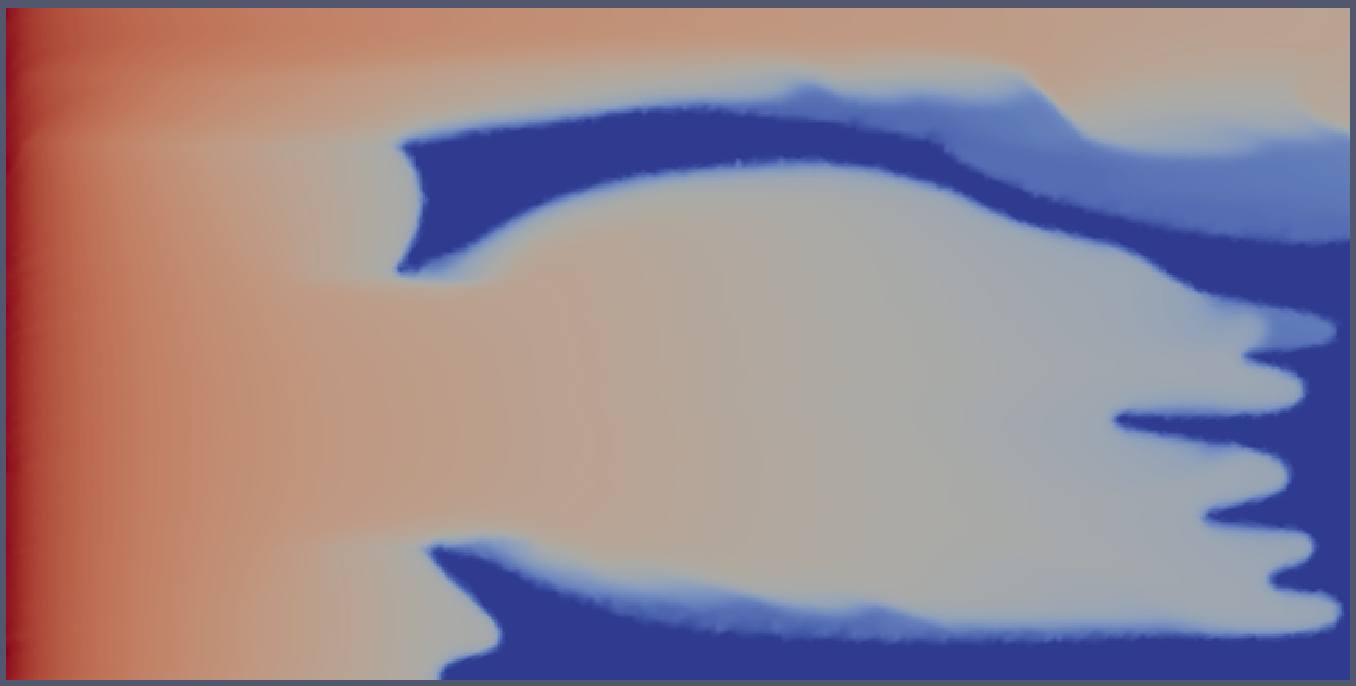
\includegraphics[width=.65\textwidth]{./Pics1/mr10_5regions_fixed/5regions_fixed_1500.pdf} 
}
\vspace{0.0cm}
\hbox{\hspace{6.5cm} (a) flow at t=1500 (fixed mesh)   
}
\vspace{0.25cm}
\hbox{\hspace{3.5cm}
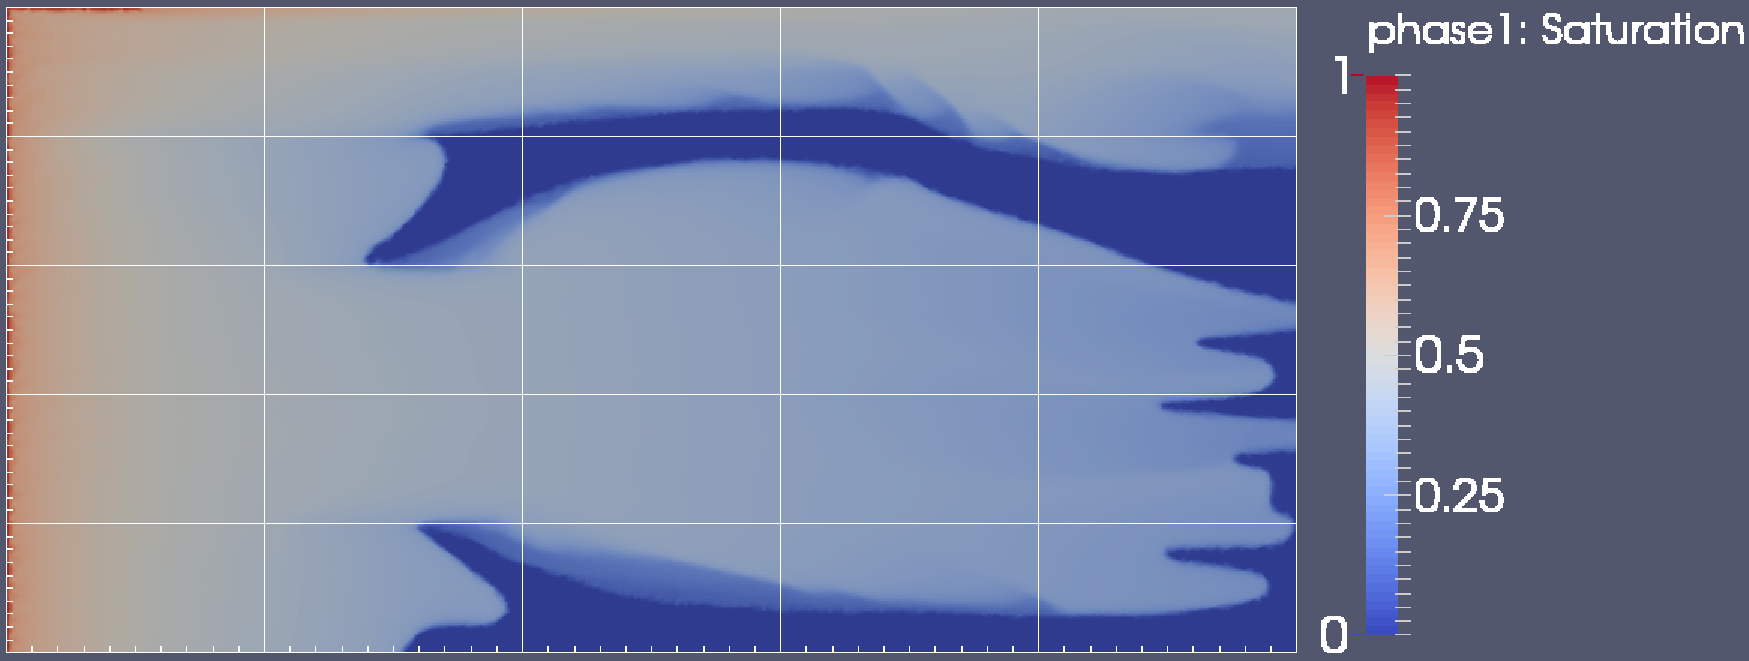
\includegraphics[width=.9\textwidth]{./Pics1/mr10_5regions_adapt/5regions_adapt_1500_1.pdf}
}
\vspace{0.0cm}
\hbox{\hspace{6.5cm} (b) flow at t=1500 (adaptive mesh)     
}
}     
\caption{At $t=0.75 sec$ ($t=1500$, timestemp) the initial cross flow is now fully developed and has travel all the way towards the outlet (right-hand side). and the finger below start forming a front that is also travelling towards the left-hand side.}
\label{fig:2testcase_c}
\end{figure}
\end{landscape}
\clearpage



%%%%
%%%%  FIGURE
%%%%
\begin{landscape}
\begin{figure}[ht] 
\vbox{
\hbox{\hspace{3.5cm}
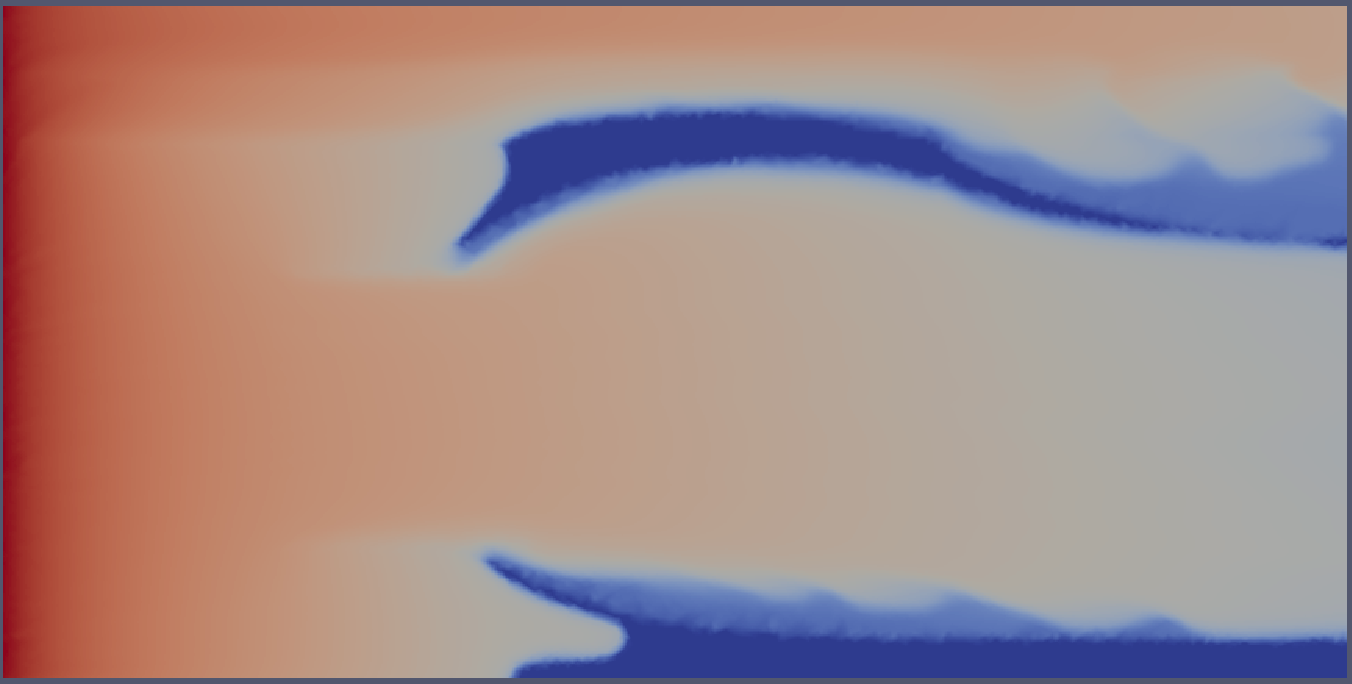
\includegraphics[width=.65\textwidth]{./Pics1/mr10_5regions_fixed/5regions_fixed_2000.pdf} 
}
\vspace{0.0cm}
\hbox{\hspace{6.5cm} (a) flow at t=end (fixed mesh)   
}
\vspace{0.25cm}
\hbox{\hspace{3.5cm}
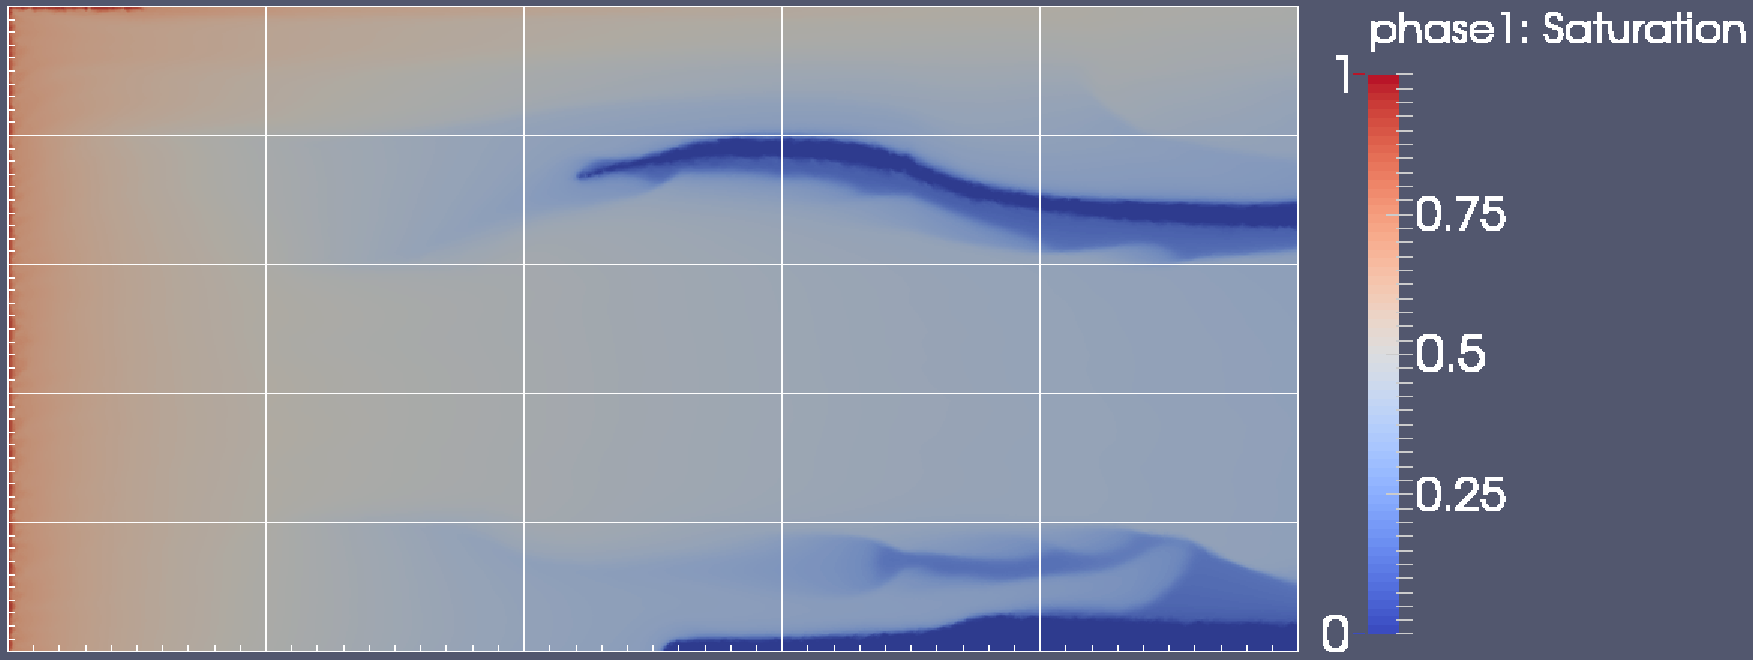
\includegraphics[width=.9\textwidth]{./Pics1/mr10_5regions_adapt/5regions_adapt_3000_1.pdf}
}
\vspace{0.0cm}
\hbox{\hspace{6.5cm} (b) flow at t=end (adaptive mesh)     
}
}     
\caption{Using the $P_{1}DGP_{2}$ element type for VR=$10$ under the same time steps, we compared the impact of fixed and adaptive mesh for the same timeframe. The end of simulation happens at $time=5 sec$ and for the timestemp $t=9999$ while the number of elements in both simulations was approximately $4700$. When adaptive mesh is introduce there is better repersentation of the fluid instabilities as these are developed on time.}
\label{fig:2testcase_d}
\end{figure}
\end{landscape}
\clearpage



%%%%
%%%%  FIGURE
%%%%
\begin{landscape}
\begin{figure}[ht] 
\vbox{
\hbox{\hspace{3.5cm}
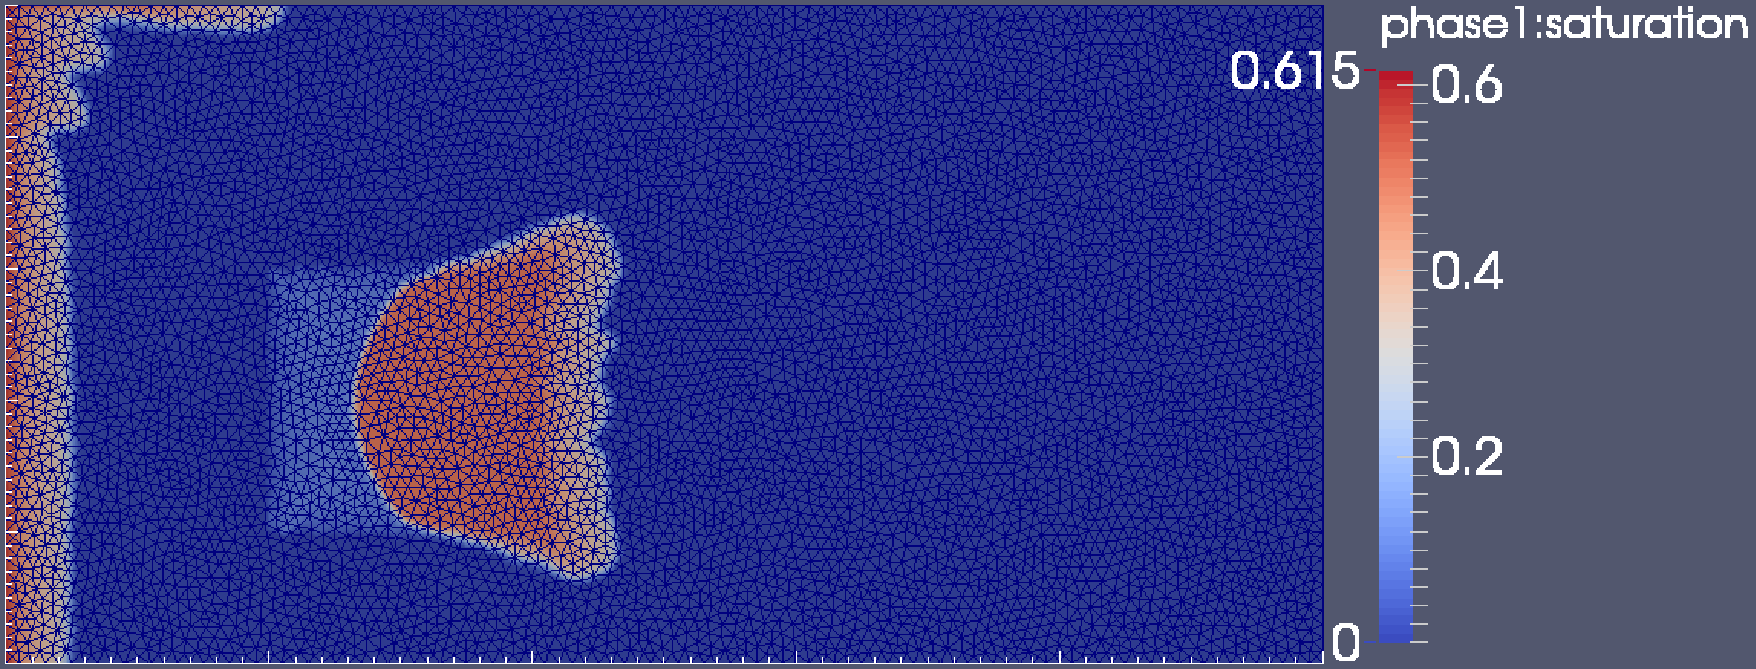
\includegraphics[width=.9\textwidth]{./Pics1/mr10_5regions_fixed_dinlet/5regions_dinlet_fixed_100_1.pdf}
}
\vspace{0.0cm}
\hbox{\hspace{6.5cm} (a) double inlet - fixed mesh   
}
\hbox{\hspace{3.5cm}
  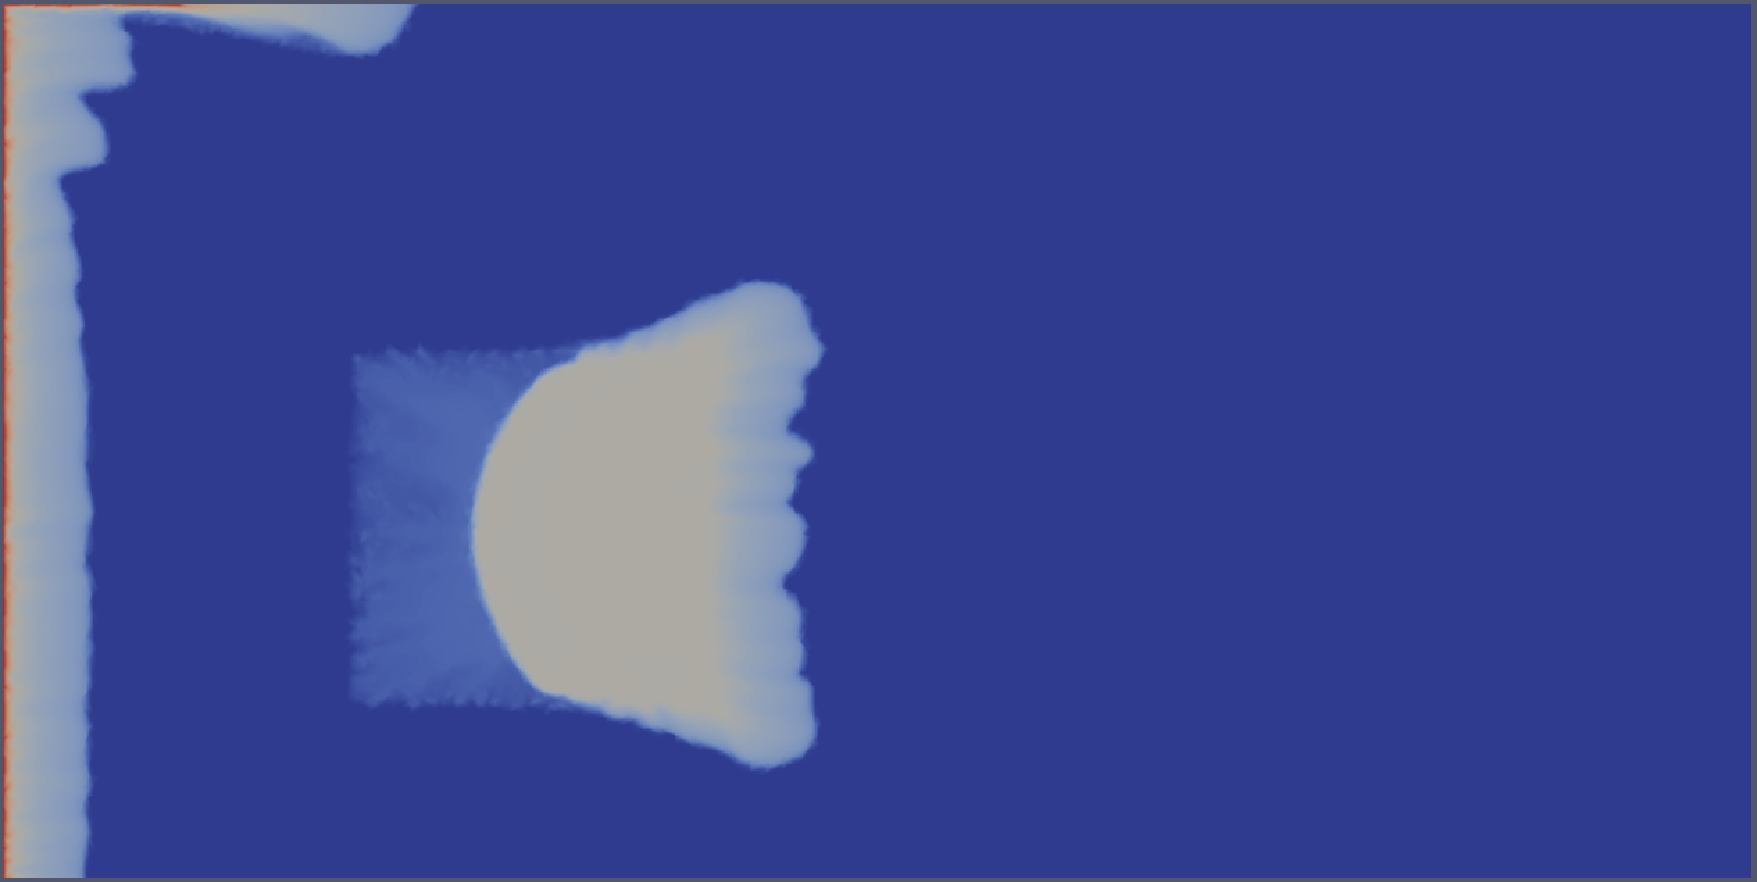
\includegraphics[width=.67\textwidth]{./Pics1/mr10_5regions_adapt_dinlet/5regions_dinlet_adapt_start.pdf}
}
\vspace{0.0cm}
\hbox{\hspace{6.5cm} (b) double inlet adaptive mesh   
}
}     
\caption{Comparing test-cases of fixed and adaptive mesh while a second region/inlet is introduced. For $t=0.101$s, using the $P_{1}DGP_{2}$ element type for MR=$10$ under the same time steps. For this simulation there are $13226$ elements for the fixed messh and $43716$ for the adaptive.}
\label{fig:3testcase_a}
\end{figure}
\end{landscape}
\clearpage

%%%%
%%%%  FIGURE
%%%%
\begin{figure}[ht] 
\vbox{
\hbox{\hspace{3.5cm}
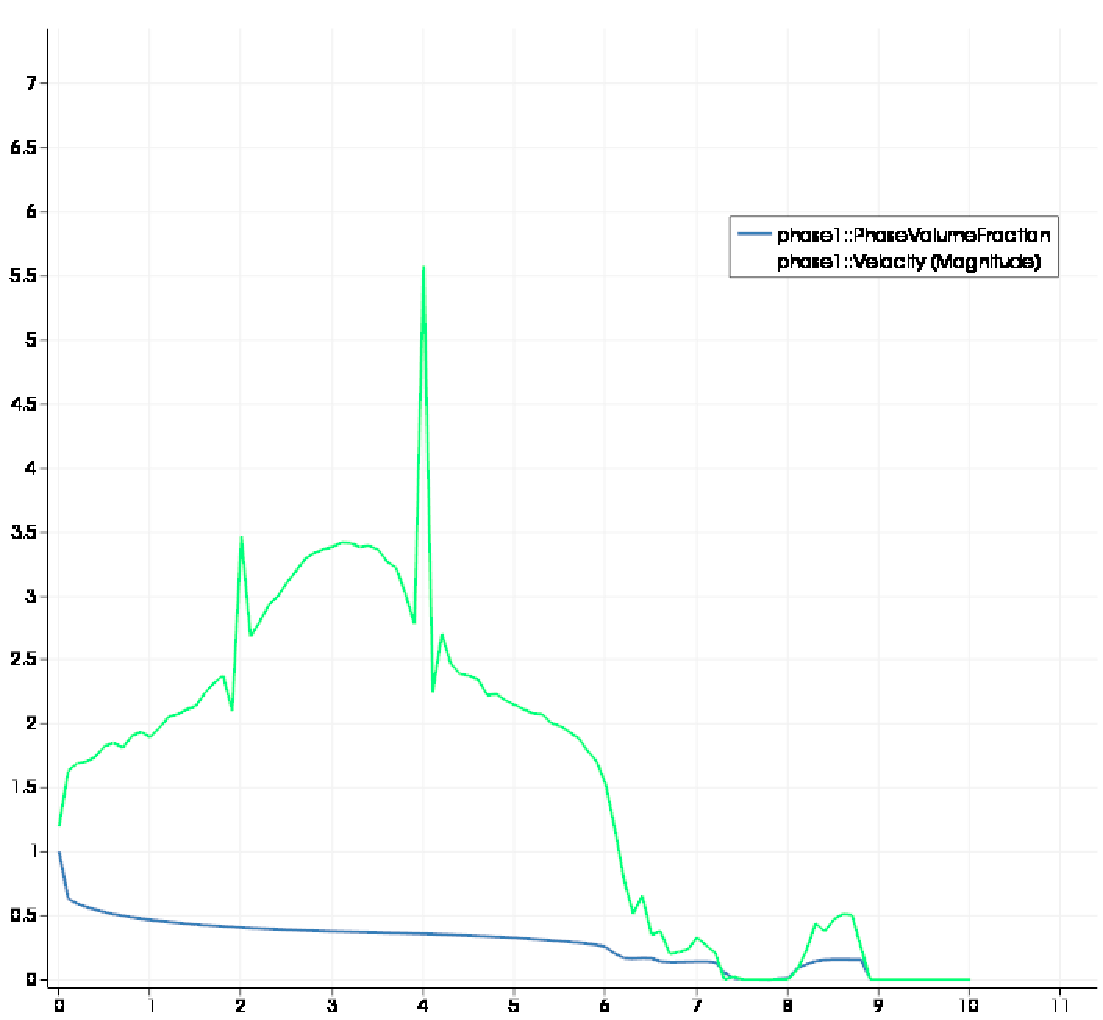
\includegraphics[width=.5\textwidth]{./Pics1/mr10_5regions_adapt/5regions_adapt_vel_magn.pdf} 
}
\vspace{0.0cm}
\hbox{\hspace{5.0cm} (a) single inlet velocity magnitude   
}
\hbox{\hspace{3.5cm}
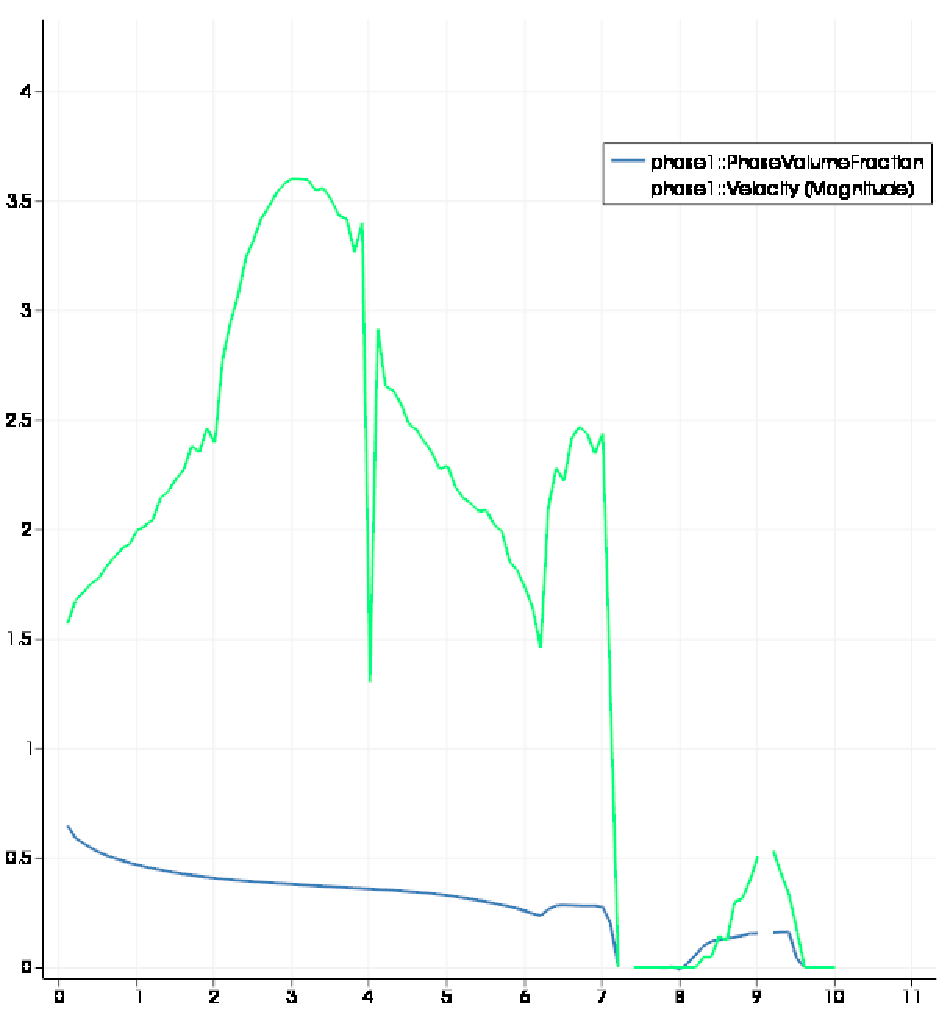
\includegraphics[width=.5\textwidth]{./Pics1/mr10_5regions_adapt_dinlet/5regions_dinlet_adapt_vel_magn.pdf}
}
\vspace{0.0cm}
\hbox{\hspace{5.0cm} (b) double inlet velocity magnitude   
}
}     
\caption{For the same time step, t=1000, these plots describe the velocity magnitudes of the phase $1$ (injected fluid) under the same boundary and initiall conditions. From top to bottom,these graphs describe the velocity magnitude %for fixed mesh is plotted(top), the velocity magnitude 
for adaptive mesh-single inlet (top) and the velocity magnitude for adaptive mesh with double inlet (bottom) as these are also presented in fig.\ref{fig:3testcase_a}. The main difference between the upper and lower plot %is not just the ability to capture in greater detail, the fluid instabilities as they happenduring the finger development and their velocity patterns. While there 
is the impact of the second injection interval as this can be seen from the slope and the rate that the velocity magnitude is changing.}
\label{fig:vel_magn}
\end{figure}

%%%%
%%%%  FIGURE
%%%%
\begin{landscape}
\begin{figure}[ht] 
\vbox{
\hbox{\hspace{3.5cm}
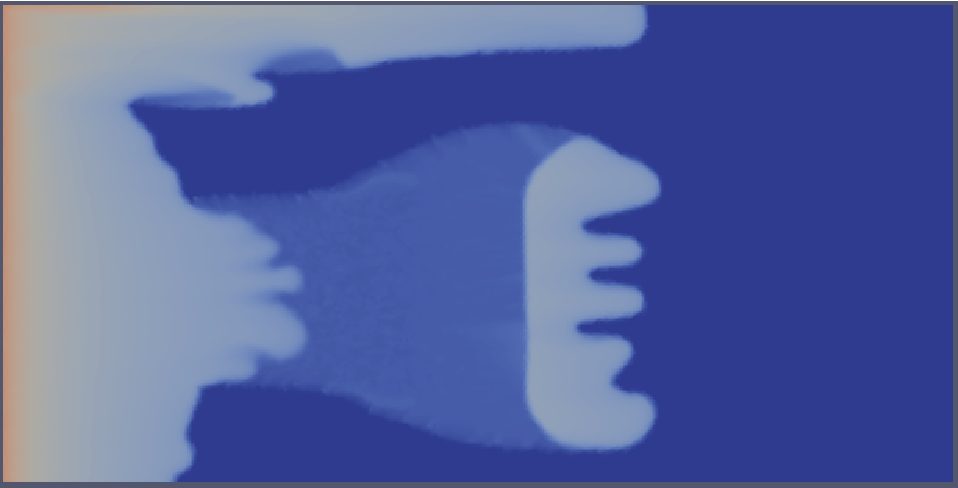
\includegraphics[width=.65\textwidth]{./Pics1/5reg_dinlet_fixed_500.pdf} 
}
\vspace{0.0cm}
\hbox{\hspace{6.5cm} (a) double inlet - fixed mesh   
}
\hbox{\hspace{3.5cm}
\includegraphics[width=.9\textwidth]{./Pics1/5reg_dinlet_adapt_500_1.pdf}
}
\vspace{0.0cm}
\hbox{\hspace{6.5cm} (b) double inlet adaptive mesh   
}
}     
\caption{For $t=5$s there is a comparison between fixed mesh(a) and adaptive mesh(b).}
\label{fig:3testcase_b}
\end{figure}
\end{landscape}
\clearpage

%%%%
%%%%  FIGURE
%%%%
\begin{landscape}
\begin{figure}[ht] 
\vbox{
\hbox{\hspace{3.5cm}
\includegraphics[width=.65\textwidth]{./Pics1/5reg_dinlet_fixed_1500.pdf} 
}
\vspace{0.0cm}
\hbox{\hspace{6.5cm} (a) double inlet - fixed mesh   
}
\hbox{\hspace{3.5cm}
\includegraphics[width=.9\textwidth]{./Pics1/5reg_dinlet_adapt_1500_1.pdf}
}
\vspace{0.0cm}
\hbox{\hspace{6.5cm} (b) double inlet adaptive mesh   
}
}     
\caption{For $t=7.5$s this is a comparison between fixed mesh(a) and adaptive mesh(b).}
\label{fig:3testcase_c}
\end{figure}
\end{landscape}
\clearpage

%%%%
%%%%  FIGURE
%%%%
\begin{landscape}
\begin{figure}[ht] 
\vbox{
\hbox{\hspace{3.5cm}
\includegraphics[width=.65\textwidth]{./Pics1/5reg_dinlet_fixed_end.pdf} 
}
\vspace{0.0cm}
\hbox{\hspace{6.5cm} (a) double inlet - fixed mesh   
}
\hbox{\hspace{3.5cm}
\includegraphics[width=.9\textwidth]{./Pics1/5reg_dinlet_adapt_end_1.pdf}
}
\vspace{0.0cm}
\hbox{\hspace{6.5cm} (b) double inlet adaptive mesh   
}
}     
\caption{This is a comparison between fixed mesh(a) and adaptive mesh(b) at the end of the simulation. For the fixed mesh at this point the maximum number of point is $13226$ while for the adaptive mesh is $7582$ and most of them are located where is needed in the domain.}
\label{fig:3testcase_d}
\end{figure}
\end{landscape}
\clearpage

%%%%
%%%%  FIGURE
%%%%
\begin{landscape}
\begin{figure}[ht] 
\vbox{
\hbox{\hspace{3.5cm}
\includegraphics[width=.8\textwidth]{./Pics1/mr100_fixed/mr100_fixed_500.pdf} 
}
\vspace{0.0cm}
\hbox{\hspace{4.0cm} (a) fixed and unstructured mesh for MR = 100 (start)   
}
\hbox{\hspace{3.5cm}
\includegraphics[width=.8\textwidth]{./Pics1/mr100_fixed/mr100_fixed_1500.pdf}
}
\vspace{0.0cm}
\hbox{\hspace{3.75cm} (b) fixed and unstructured mesh for MR = 100 (t = 1500)   
}
}     
\caption{For the case of VR=$100$ from top to bottom, the number of elements is $4680$ and fixed and unstructured mesh for the same time steps, t=$0.25$ or t=500(a), t=$0.75$ or t=1500(b). }
\label{fig:4testcase_a}
\end{figure}
\end{landscape}
\clearpage

%%%%
%%%%  FIGURE
%%%%
\begin{landscape}
\begin{figure}[ht] 
\vbox{
\hbox{\hspace{3.5cm}
\includegraphics[width=.8\textwidth]{./Pics1/mr100_fixed/mr100_fixed_3000.pdf} 
}
\vspace{0.0cm}
\hbox{\hspace{3.75cm} (c) fixed and unstructured mesh for MR = 100    
}
\hbox{\hspace{3.5cm}
\includegraphics[width=.8\textwidth]{./Pics1/mr100_fixed/mr100_fixed_end.pdf}
}
\vspace{0.0cm}
\hbox{\hspace{7.cm} (d) end of simulations     
}
}     
\caption{screenshot (c) is for t=$1.5$ sec or t=$3000$ and screenshot (d) is for t=$3.175$ sec, at the end of the simulations. }
\label{fig:4testcase_b}
\end{figure}
\end{landscape}
\clearpage





%%%
%%%  FIGURE 
%%%
\begin{figure}[h]
\begin{center}
\includegraphics[width=1.\textwidth]{diagrams/bl-exact-meth-upwind.eps}
\end{center}
\caption{Buckley--Leverett test-cases: Saturation solutions for the continuous upwind method for different 1D P$_{1}$DG-P$_{2}$ mesh  resolutions and comparison against standard analytical solution.
\label{bl-exact-meth-upwind}}
\end{figure}

%%%
%%%
%%%  FIGURE 
%%%
\begin{figure}[h]
  %\begin{center}
\vbox{\hbox{\hspace{2.5cm}
    \includegraphics[width=0.62\textwidth]{diagrams/BL_1d_P0DGP1_convergence.eps}}
\vspace{-.0cm}\hbox{\hspace{2.5cm}
    \includegraphics[width=0.62\textwidth]{diagrams/BL_1d_P1DGP2_convergence.eps}}
\vspace{-.0cm}\hbox{\hspace{2.5cm}
    \includegraphics[width=0.62\textwidth]{diagrams/BL_1d_P2DGP3_convergence.eps}}}
   % \includegraphics[width=0.45\textwidth]{BL_2d_P1DGP2_convergence}
    \caption{Buckley--Leverett test-cases: Saturation profiles for a number of element-pairs and numerical resolutions in 1D -- P$_{0}$DG-P$_{1}$ (top), P$_{1}$DG-P$_{2}$ and P$_{2}$DG-P$_{3}$ (bottom).\label{fig:BL_profiles}}
  %\end{center}
\end{figure}

%%%
%%%  FIGURE 
%%%
\begin{figure}[h]
\vbox{\hbox{\hspace{1.cm}
    \includegraphics[width=0.8\textwidth]{diagrams/L1_convergence_rate.eps}}
\vspace{.0cm}\hbox{\hspace{1.cm}
    \includegraphics[width=0.8\textwidth]{diagrams/L2_convergence_rate.eps}}}
    \caption{Buckley--Leverett test-cases: L1 (top) and L2 (bottom) error convergence rates for a number of element pairs. \label{fig:BL_converg-rates}}
\end{figure}

%%%
%%%  FIGURE 
%%%
\begin{figure}[h]
\begin{center}
\includegraphics[width=1.\textwidth]{diagrams/bl-upwind-v-up-and-down.eps}
\end{center}
\caption{Buckley--Leverett test-cases: Comparison of the optimal upwind formulation when using upwinding (OU) and coupled upwind/downwind (OU-D). The finite element interpolation of the saturation field $\left(S_{1}\right)$ is shown at different mesh resolutions. Downwind seems to detract from the accuracy of the solution. \label{bl-upwind-v-up-and-down}}
\end{figure}

%%%
%%%  FIGURE 
%%%
\begin{figure}[h]
\vbox{
\begin{center}
\includegraphics[width=1.\textwidth]{diagrams/bl-exact-meth-cv-0-8-ele50.eps}
\end{center}
\vspace{0.cm}}
\caption{Buckley--Leverett test-cases: Comparison of control volume
  solutions using 80$\%$ upwinding and with optimal upwinding and
  using 50 continuous P$_{1}$DG-P$_{2}$
  elements. \label{bl-exact-meth-cv-0-8-ele50}}
\end{figure}

%%%
%%%  FIGURE 
%%%
\begin{figure}[h]
\begin{center}
\includegraphics[width=1.\textwidth]{diagrams/bl-dg-2eles.eps}
\end{center}
\caption{Buckley--Leverett test-cases: Two element solution using the
  discontinuous formulation. Saturation field from both CV solution
  and FEM interpolation are shown.  \label{bl-dg-2eles}}
\end{figure}

%%%
%%%  FIGURE 
%%%
\begin{figure}[h]
\vbox{
\hbox{\hspace{.3cm}\includegraphics[width=.9\textwidth]{diagrams/bl-dg-4-10-20.eps}}
\vspace{-0.cm}
\hbox{\hspace{.3cm}\includegraphics[width=.9\textwidth]{diagrams/bl-dg-cent-4-10-20.eps}}}
\caption{Buckley--Leverett test-cases: Saturation field obtained from
  the discontinuous and continuous formulation with different mesh
  resolutions. Solutions with (top) and without (bottom) upwinding
  scheme. Notice that oscillations are suppressed with the upwinding
  scheme.\label{bl-dg-cent-4-10-20}}
\end{figure}


%%%
%%%  FIGURE 
%%%
\begin{figure}[h]
\vbox{
\hbox{\hspace{.3cm}\includegraphics[width=.9\textwidth]{diagrams/bl-dg-4-10-vers-cty.eps}}
\vspace{-0.cm}
\hbox{\hspace{.3cm}\includegraphics[width=.9\textwidth]{diagrams/bl-dg-p1-2-4-5-10-20-40.eps}}}
\caption{Buckley--Leverett test-cases: Saturation field obtained from
  (top) continuous and discontinuous (between elements) formulations
  (solution with 50 elements may be considered as a converged
  result). Solution obtained (bottom) from linear pressure (P1)
  formulation with different mesh resolution with comparison against
  P2-pressure formulation (continuous). \label{bl-dg-4-10-vers-cty}}
\end{figure}


%%%
%%%  FIGURE 
%%%
\begin{figure}[H]
\vbox{
\begin{center}
\includegraphics[width=17.5cm,height=12.5cm]{diagrams/bl-dg-4-10-vers-cty}
\end{center}
\vspace{0.cm}}
\caption{Gas saturations shown comparing the accuracy of the
  discontinuous between elements and continuous formulation. The 50
  element continuous solution may be viewed as a converged result.  }
\label{bl-dg-4-10-vers-cty}
\end{figure}

\begin{comment}
%%%
%%%  FIGURE 
%%%
\begin{figure}[h]
\vbox{
\hbox{\hspace{.2cm}
    \includegraphics[width=1.\textwidth]{diagrams/map_2d.png}}
\vspace{1.cm}
\hbox{\hspace{0.2cm}
    \includegraphics[width=1.\textwidth]{./diagrams/map_3d.png}}}
    \caption{Buckley-Leverett test-cases: phase 1 saturation surface maps for a 2- (770 triangles) and 3-D (1207 tetrahedra) simulations (\PN[1]{2} unstructured mesh grids) at time $t=0.5$. \label{fig:maps2d_3d}}
\end{figure}


%%%  FIGURE 
%%%
\begin{figure}[h]
\vbox{\hbox{\hspace{.3cm}
    \includegraphics[width=0.9\textwidth]{diagrams/BL_2d_P1DGP2_convergence.eps}}
\vspace{-.0cm}\hbox{\hspace{.3cm}
    \includegraphics[width=0.9\textwidth]{./diagrams/simulations_2d_3d.eps}}}
    \caption{Buckley-Leverett test-cases: 2- and 3-D phase 1 saturation profiles with \PN[1]{2} elements. Sensitivity analysis for (top) grid resolution using structured \PN[1]{2} mesh, and (bottom) mesh type.\label{fig:BL_2d_profiles}}
\end{figure}

\end{comment}



\end{document}

%%
%% End of tex file.

%%  LocalWords:  checkboard
